\documentclass[12pt,a4paper,oneside]{report} %<<<1 ------------------------------
% fonts, encoding:
\usepackage[utf8]{inputenc}             % file is in utf8:
\usepackage{cmap}                       % pdf is created with correct special characters, requires proper font, see next two lines
\usepackage[T1]{fontenc}                % see higher line
\usepackage{tgtermes}                   % high quality times font
\usepackage{textcomp}                   % proper micro sign for SI, use: \textmu, in equation: $\hbox{\textmu}$
\usepackage{slantsc}                   % proper micro sign for SI, use: \textmu, in equation: $\hbox{\textmu}$
\usepackage{calc}                   % provides \widthof
\usepackage{enumitem}                   % provides \begin{description} with settings []
\usepackage{color}                   % provides coloured text
% obrazky:
\usepackage{graphicx}                   % to insert pictures
\usepackage{grffile}                    % enables spaces in picture file names
\grffilesetup{ multidot=false, babel=false, encoding, inputencoding=utf8, filenameencoding=utf8, space=true}
\newcommand*{\FILEDOT}{.}                   % if picture file name containt dot (e.g. aaa.bbb.pdf), then TeX considers rest as filename extension, so dot must be written as follows: \includegraphics{aaa\FILEDOT bbb.eps}
% rest:
\usepackage[pdftex,
            unicode,
            pdfauthor={Q-Wave consorcium},
            pdftitle={QWTB documentation: implemented algorithms},
            pdfkeywords={algorithm, data procesing, sampling, toolbox},
            pdfproducer={Latex with hyperref},
            pdfcreator={pdflatex}]{hyperref}
%\usepackage[a4paper]{geometry}          % ensure A4
%\geometry{verbose,lmargin=2.5cm,rmargin=2.5cm,tmargin=2.5cm,bmargin=2.5cm}      % margins settings
\usepackage{url}                        % enables \url in bibtex
%\usepackage{setspace} \doublespacing   % double line spacing, for 1.5 set \onehalfspace
\usepackage{xspace}                     % proper automatic spacing after user defined commands
\usepackage{amsmath}                    % better equations

% chapter/section settings %<<<1 ----------------------------------------------------
\usepackage{titlesec}
%\titleformat*{\section}{\color{blue}{\itshape}}
\titleformat{\chapter}[display]
{\normalfont\bfseries\Huge\filcenter}
{}
{-0.5em}
{}

\titleformat{\section}[display]
{\normalfont\Large\filcenter}
{}
{-0.75em}
{\vspace{1em}\titlerule[1pt]\vspace{0.4em}}

\pagestyle{headings}

% lstlisting settings %<<<1 ----------------------------------------------------
\usepackage{listings}                   % for source code formatting
\definecolor{mygreen}{rgb}{0,0.6,0}
\definecolor{mygray}{rgb}{0.5,0.5,0.5}
\definecolor{lightgray}{rgb}{0.95,0.95,0.95}
\definecolor{mymauve}{rgb}{0.58,0,0.82}

\lstdefinestyle{mcode}{
%\lstset{ %
  backgroundcolor=\color{lightgray},   % choose the background color; you must add \usepackage{color} or \usepackage{xcolor}
  basicstyle=\normalsize\sffamily,        % the size of the fonts that are used for the code
  breakatwhitespace=false,         % sets if automatic breaks should only happen at whitespace
  breaklines=true,                 % sets automatic line breaking
  captionpos=b,                    % sets the caption-position to bottom
  commentstyle=\color{mygreen},    % comment style
  deletekeywords={...},            % if you want to delete keywords from the given language
  escapeinside={\%*}{*)},          % if you want to add LaTeX within your code
  extendedchars=true,              % lets you use non-ASCII characters; for 8-bits encodings only, does not work with UTF-8
  frame=single,	                   % adds a frame around the code
  keepspaces=true,                 % keeps spaces in text, useful for keeping indentation of code (possibly needs columns=flexible)
  keywordstyle=\color{blue},       % keyword style
  language=Matlab,                 % the language of the code
  otherkeywords={*,qwtb,alg_info,alg_wrapper,
        normrnd, alg_test,alg_example,...},           % if you want to add more keywords to the set
  numbers=none,                    % where to put the line-numbers; possible values are (none, left, right)
  numbersep=5pt,                   % how far the line-numbers are from the code
  numberstyle=\tiny\color{mygray}, % the style that is used for the line-numbers
  rulecolor=\color{black},         % if not set, the frame-color may be changed on line-breaks within not-black text (e.g. comments (green here))
  showspaces=false,                % show spaces everywhere adding particular underscores; it overrides 'showstringspaces'
  showstringspaces=false,          % underline spaces within strings only
  showtabs=false,                  % show tabs within strings adding particular underscores
  stepnumber=2,                    % the step between two line-numbers. If it's 1, each line will be numbered
  stringstyle=\color{mymauve},     % string literal style
  tabsize=2,                       % sets default tabsize to 2 spaces
  title=\lstname,                  % show the filename of files included with \lstinputlisting; also try caption instead of title
  belowskip=0pt                  % skip after end of lstlistings
}

\lstdefinestyle{output}{
%\lstset{ %
  backgroundcolor=\color{lightgray},   % choose the background color; you must add \usepackage{color} or \usepackage{xcolor}
  basicstyle=\normalsize\itshape,        % the size of the fonts that are used for the code
  breakatwhitespace=false,         % sets if automatic breaks should only happen at whitespace
  breaklines=true,                 % sets automatic line breaking
  captionpos=b,                    % sets the caption-position to bottom
  commentstyle=\color{mygreen},    % comment style
  deletekeywords={...},            % if you want to delete keywords from the given language
  escapeinside={\%*}{*)},          % if you want to add LaTeX within your code
  extendedchars=true,              % lets you use non-ASCII characters; for 8-bits encodings only, does not work with UTF-8
  frame=none,	                   % adds a frame around the code
  keepspaces=true,                 % keeps spaces in text, useful for keeping indentation of code (possibly needs columns=flexible)
  keywordstyle=\color{blue},       % keyword style
  language=Matlab,                 % the language of the code
  otherkeywords={*,qwtb,alg_info,alg_wrapper,alg_test,alg_example,...},           % if you want to add more keywords to the set
  numbers=none,                    % where to put the line-numbers; possible values are (none, left, right)
  numbersep=5pt,                   % how far the line-numbers are from the code
  numberstyle=\tiny\color{mygray}, % the style that is used for the line-numbers
  rulecolor=\color{black},         % if not set, the frame-color may be changed on line-breaks within not-black text (e.g. comments (green here))
  showspaces=false,                % show spaces everywhere adding particular underscores; it overrides 'showstringspaces'
  showstringspaces=false,          % underline spaces within strings only
  showtabs=false,                  % show tabs within strings adding particular underscores
  stepnumber=2,                    % the step between two line-numbers. If it's 1, each line will be numbered
  stringstyle=\color{mymauve},     % string literal style
  tabsize=2,                       % sets default tabsize to 2 spaces
  title=\lstname,                  % show the filename of files included with \lstinputlisting; also try caption instead of title
  belowskip=0pt,                  % skip after end of lstlistings
  xleftmargin=20pt                      % margin on left side
}

\lstset{style=mcode}
     % user defined code formatting

% bibliography settings %<<<1 ----------------------------------------------------
\usepackage[english]{babel} % main language of the document must be last
\usepackage[
   backend=biber      % if we want unicode 
  ,style=ieee   % or iso-numeric for numeric citation method          
  ,babel=other        % to support multiple languages in bibliography
  %,sortlocale=cs_CZ   % locale of main language, it is for sorting
  ,sortlocale=en_UK   % locale of main language, it is for sorting
  ,bibencoding=UTF8   % this is necessary only if bibliography file is in different encoding than main document
]{biblatex}

% \bibliography{alllib2}
%\defbibenvironment{bibliography}
%    {\list
%        {[\printfield[labelnumberwidth]{labelnumber}]}
%        {\setlength{\labelwidth}{\labelnumberwidth}
%        \setlength{\leftmargin}{4pt}
%        \setlength{\labelsep}{10pt}
%        \addtolength{\leftmargin}{\labelsep}
%        \setlength{\itemsep}{6pt}
%        \setlength{\parsep}{\bibparsep}}
%        \renewcommand*{\makelabel}[1]{\hss##1}}
%    {\endlist}
%    {\item}

% shorts: %<<<1 ----------------------------------------------------

\def\Alg{{\sc Algorithm}\xspace}
\def\Algs{{\sc Algorithms}\xspace}
\def\Tb{{\sc Toolbox}\xspace}
\def\Da{{\sc Data}\xspace}
\def\Mea{{\sc Measurement}\xspace}
\def\Qua{{\sc Quantity}\xspace}
\def\Quas{{\sc Quantities}\xspace}
\def\Wr{{\sc Wrapper}\xspace}
\def\Wrs{{\sc Wrappers}\xspace}
\def\matlab{{\sc MATLAB}\xspace}
\def\octave{{\sc GNU Octave}\xspace}
\def\labview{{\sc LabVIEW}\xspace}
\def\mgo{\matlab/\octave\xspace}
        
\begin{document} % other document settings --------------------------------------------%<<<1
% how to devide special words, e.g. auto-mation
\hyphenation{Frame-work OpenOffice SourceForge Windows}
%\def\thesection{\Roman{section}}       % redefines numbering style of sections
\renewcommand\floatpagefraction{.9} \renewcommand\topfraction{.9} \renewcommand\bottomfraction{.9} \renewcommand\textfraction{.1} \setcounter{totalnumber}{50} \setcounter{topnumber}{50} \setcounter{bottomnumber}{50} % if too many pictures, change text/float fraction
\renewcommand{\labelitemi}{--}          % item sepparator
\setlength{\unitlength}{1mm}            % default length in picture environment

% tight description environment:
\newenvironment{tightdesc}{\begin{description}[itemsep=0pt]} 
                              {\end{description}}

% names of sections:
\def\infosection{Description}
\def\examplesection{Example}
% remove "chapter" from chapter heading:
\renewcommand{\chaptername}{}

\title{QWTB documentation: implemented algorithms}
\author{Q-Wave consorcium}

% first page ----------------------------------------------------------------------- %<<<1 ------------------------------
\thispagestyle{empty}
\begin{center}
        \vspace*{10em}
        {\huge
        
\includegraphics[width=0.3\textwidth]{logo/qwtb_logo.png}

        \vspace{2.0em}
        QWTB documentation\\

        \vspace{1.5em}
        Implemented algorithms}\\

        \vfill
        {\Large \color{red}{QWTB version 0.2}}

        \vspace{1em}
        {\Large \url{https://qwtb.github.io/qwtb/}}
\end{center}
\newpage

\tableofcontents

\chapter{Introduction} %<<<1 ------------------------------
This document gives overview of the algorithms implemented in toolbox QWTB.

Toolbox was realized within the EMRP-Project SIB59 Q-Wave. The EMRP is jointly funded by the EMRP
par- ticipating countries within EURAMET and the European Union.

\vspace{4em}

\includegraphics[width=0.3\textwidth]{sources/Q-Wave_logo_01.pdf}
\hfill

\includegraphics[width=0.3\textwidth]{sources/eurametlogo.jpg}

% testing algorithms - normally commented: %<<<1 ------------------------------
% \chapter{testG -- testG} 
% % included files are automatically generated by info_all_algs.m script and by Matlab publish
% % function and converted by bash script betterpublish.
% \section*{\infosection}
% \begin{tightdesc}
\item [Id:] testG
\item [Name:] Test with GUF
\item [Description:] Calculates maximum value of the measured record
\item [Citation:] see EMRP Q-Wave
\item [Remarks:] Do not use. This is only for testing QWTB
\item [License:] MIT License
\item [Provides GUF:] yes
\item [Provides MCM:] no
\item [Input Quantities] \rule{0em}{0em}
    \begin{tightdesc}
    \item [Required:] 
        \textsf{x},\enspace \textsf{y}
    \item [Descriptions:] \rule{0em}{0em}
        \begin{tightdesc}
            \item[\textsf{x}] -- independent quantity
            \item[\textsf{y}] -- dependent quantity
        \end{tightdesc}
    \end{tightdesc}
\item [Output Quantities:] \rule{0em}{0em}
    \begin{tightdesc}
        \item[\textsf{max}] -- maximal dependent quantity
        \item[\textsf{min}] -- minimal dependent quantity
    \end{tightdesc}
\end{tightdesc}

% \section*{\examplesection}
% 
% This LaTeX was auto-generated from an M-file by MATLAB.
% To make changes, update the M-file and republish this document.

%%% \documentclass{article}
%%% \usepackage{graphicx}
%%% \usepackage{color}

%%% \sloppy
%%% \definecolor{lightgray}{gray}{0.5}
\setlength{\parindent}{0pt}

%%% \begin{document}

    
    
\subsection*{testG}

\begin{par}
Example for algorithm testG. Algorithm is usefull only for testing QWTB toolbox. It calculates maximal and minimal value of the record. GUF is calculated by wrapper.
\end{par} \vspace{1em}
\begin{par}
See also \lstinline{qwtb}
\end{par} \vspace{1em}

\subsubsection*{Contents}

\begin{itemize}
\setlength{\itemsep}{-1ex}
   \item Generate sample data
   \item Call algorithm
   \item Plot results
\end{itemize}


\subsubsection*{Generate sample data}

\begin{par}
Two quantities are prepared: \lstinline{x} and \lstinline{y}.
\end{par} \vspace{1em}
\begin{lstlisting}[style=mcode]
x = []; y = [];
x.v = [1:20];
y.v = [1:14 13:-1:8];
\end{lstlisting}
\begin{par}
All uncertainties are set to 1.
\end{par} \vspace{1em}
\begin{lstlisting}[style=mcode]
x.u = x.v.*0 + 1;
y.u = y.v.*0 + 1;
\end{lstlisting}
\begin{par}
Set degrees of freedom.
\end{par} \vspace{1em}
\begin{lstlisting}[style=mcode]
x.d = x.v.*0 + 60;
y.d = y.v.*0 + 9;
\end{lstlisting}
\begin{par}
Quantities are put into data input structure \lstinline{DI}.
\end{par} \vspace{1em}
\begin{lstlisting}[style=mcode]
DI = [];
DI.x = x;
DI.y = y;
\end{lstlisting}
\begin{par}
Create calculation settings \lstinline{CS} and set uncertainty calculation method to GUM uncertainty framework.
\end{par} \vspace{1em}
\begin{lstlisting}[style=mcode]
CS = [];
CS.unc = 'guf';
\end{lstlisting}


\subsubsection*{Call algorithm}

\begin{par}
Use QWTB to apply algorithm \lstinline{testG} to data \lstinline{DI} with calculation settings \lstinline{CS}.
\end{par} \vspace{1em}
\begin{lstlisting}[style=mcode]
DO = qwtb('testG', DI, CS);
\end{lstlisting}

        \begin{lstlisting}[style=output]
QWTB: default correlation matrix generated for quantity `x`
QWTB: default correlation matrix generated for quantity `y`
QWTB: uncertainty calculation by means of wrapper or algorithm
\end{lstlisting} \color{black}
    

\subsubsection*{Plot results}

\begin{par}
Plot input data and calculated maximal and minimal values as a red and green lines with uncertainties represented by dashed lines.
\end{par} \vspace{1em}
\begin{lstlisting}[style=mcode]
figure
hold on
errorbar(DI.x.v, DI.y.v, DI.y.u, 'xb')
plot([DI.x.v(1) DI.x.v(end)], [DO.max.v DO.max.v], '-r', 'linewidth', 3)
plot([DI.x.v(1) DI.x.v(end)], [DO.max.v - DO.max.u DO.max.v - DO.max.u], '--r', 'linewidth', 3)
plot([DI.x.v(1) DI.x.v(end)], [DO.min.v DO.min.v], '-g', 'linewidth', 3)
plot([DI.x.v(1) DI.x.v(end)], [DO.min.v - DO.min.u DO.min.v - DO.min.u], '--g', 'linewidth', 3)
plot([DI.x.v(1) DI.x.v(end)], [DO.max.v + DO.max.u DO.max.v + DO.max.u], '--r', 'linewidth', 3)
plot([DI.x.v(1) DI.x.v(end)], [DO.min.v + DO.min.u DO.min.v + DO.min.u], '--g', 'linewidth', 3)
legend('original data (DI.x.v, DI.y.v)', 'line at maximum value (DO.max.v)', 'uncertainty',  'line at minimum value (DO.min.v)', 'uncertainty', 'location', 'southoutside')
xlabel('quantity x')
ylabel('quantity y')
title('input data and results of testG algorithm')
hold off
\end{lstlisting}

\begin{center}
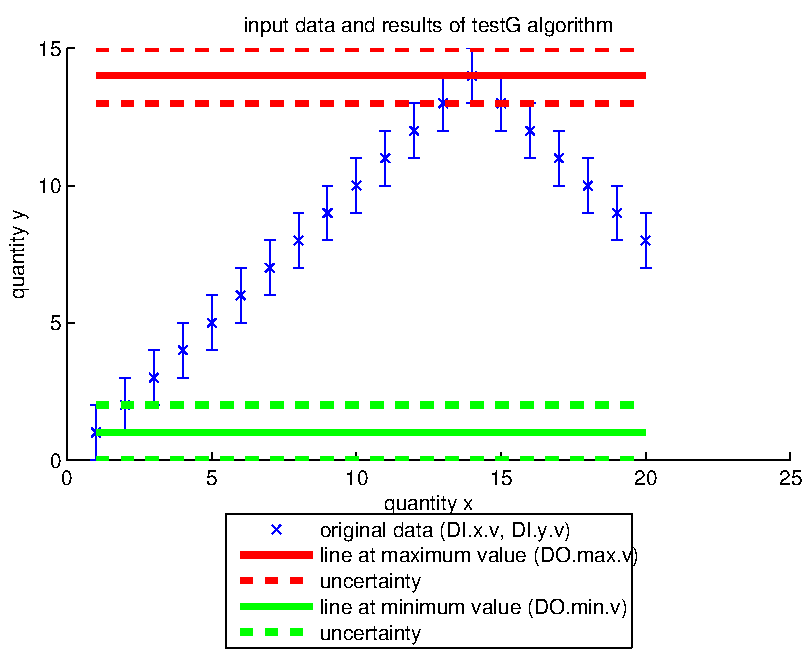
\includegraphics[width=0.7\textwidth]{algs_examples_published/testG_alg_example_01.pdf}
\end{center}



%%% \end{document}
    

% 
% \chapter{testGM -- testGM} 
% % included files are automatically generated by info_all_algs.m script and by Matlab publish
% % function and converted by bash script betterpublish.
% \section*{\infosection} 
% \begin{tightdesc}
\item [\textsf{.id}] --- testGM
\item [\textsf{.name}] --- Test with GUF and MCM
\item [\textsf{.desc}] --- Calculates maximum value of the measured record
\item [\textsf{.citation}] --- see EMRP Q-Wave
\item [\textsf{.remarks}] --- Do not use. This is only for testing QWTB
\item [\textsf{.license}] --- see license of QWTB
\item [\textsf{.requires}] \rule{0em}{0em}
\begin{tightdesc}
\item [\textsf{x}] --- independent quantity
\item [\textsf{y}] --- dependent quantity
\end{tightdesc}
\item [\textsf{.returns}] \rule{0em}{0em}
\begin{tightdesc}
\item [\textsf{max}] --- maximal dependent quantity
\item [\textsf{min}] --- minimal dependent quantity
\end{tightdesc}
\item [\textsf{.providesGUF}] --- yes
\item [\textsf{.providesMCM}] ---  yes
\end{tightdesc}

% \section*{\examplesection}
% 
% This LaTeX was auto-generated from an M-file by MATLAB.
% To make changes, update the M-file and republish this document.

%%% \documentclass{article}
%%% \usepackage{graphicx}
%%% \usepackage{color}

%%% \sloppy
%%% \definecolor{lightgray}{gray}{0.5}
\setlength{\parindent}{0pt}

%%% \begin{document}

    
    
\subsection*{testGM}

\begin{par}
Example for algorithm testGM. Algorithm is usefull only for testing QWTB toolbox. It calculates maximal and minimal value of the record. GUF/MCM is calculated by wrapper.
\end{par} \vspace{1em}
\begin{par}
See also \lstinline{qwtb}
\end{par} \vspace{1em}

\subsubsection*{Contents}

\begin{itemize}
\setlength{\itemsep}{-1ex}
   \item Generate sample data
   \item Call algorithm
   \item Plot results
\end{itemize}


\subsubsection*{Generate sample data}

\begin{par}
Two quantities are prepared: \lstinline{x} and \lstinline{y}.
\end{par} \vspace{1em}
\begin{lstlisting}[style=mcode]
x = []; y = [];
x.v = [1:20];
y.v = [1:14 13:-1:8];
\end{lstlisting}
\begin{par}
All uncertainties are set to 1.
\end{par} \vspace{1em}
\begin{lstlisting}[style=mcode]
x.u = x.v.*0 + 1;
y.u = y.v.*0 + 1;
\end{lstlisting}
\begin{par}
Set degrees of freedom.
\end{par} \vspace{1em}
\begin{lstlisting}[style=mcode]
x.d = x.v.*0 + 60;
y.d = y.v.*0 + 9;
\end{lstlisting}
\begin{par}
Quantities are put into data input structure \lstinline{DI}.
\end{par} \vspace{1em}
\begin{lstlisting}[style=mcode]
DI = [];
DI.x = x;
DI.y = y;
\end{lstlisting}
\begin{par}
Create calculation settings \lstinline{CS} and set uncertainty calculation method to Monte Carlo method. Allow randomization of uncertainties by the QWTB toolbox.
\end{par} \vspace{1em}
\begin{lstlisting}[style=mcode]
CSMCM = [];
CSMCM.unc = 'mcm';
CSMCM.mcm.randomize = 1;
\end{lstlisting}
\begin{par}
Create calculation settings and set uncertainty calculation method to GUM uncertainty framework.
\end{par} \vspace{1em}
\begin{lstlisting}[style=mcode]
CSGUF = [];
CSGUF.unc = 'guf';
\end{lstlisting}


\subsubsection*{Call algorithm}

\begin{par}
Use QWTB to apply algorithm \lstinline{testGM} to data \lstinline{DI} with calculation settings \lstinline{CSGUF}.
\end{par} \vspace{1em}
\begin{lstlisting}[style=mcode]
DOGUF = qwtb('testGM', DI, CSGUF);
\end{lstlisting}

        \begin{lstlisting}[style=output]
QWTB: default correlation matrix generated for quantity `x`
QWTB: default correlation matrix generated for quantity `y`
QWTB: uncertainty calculation by means of wrapper or algorithm
\end{lstlisting} \color{black}
    \begin{par}
Use QWTB to apply algorithm \lstinline{testGM} to data \lstinline{DI} with calculation settings \lstinline{CSMCM}.
\end{par} \vspace{1em}
\begin{lstlisting}[style=mcode]
DOMCM = qwtb('testGM', DI, CSMCM);
\end{lstlisting}

        \begin{lstlisting}[style=output]
QWTB: default correlation matrix generated for quantity `x`
QWTB: quantity x was randomized by QWTB
QWTB: default correlation matrix generated for quantity `y`
QWTB: quantity y was randomized by QWTB
QWTB: uncertainty calculation by means of wrapper or algorithm
\end{lstlisting} \color{black}
    

\subsubsection*{Plot results}

\begin{par}
Plot input data and calculated maximal and minimal values as a red and green lines with uncertainties represented by dashed lines.
\end{par} \vspace{1em}
\begin{lstlisting}[style=mcode]
figure
hold on
errorbar(DI.x.v, DI.y.v, DI.y.u, 'xb')
plot([DI.x.v(1) DI.x.v(end)], [DOGUF.max.v DOGUF.max.v], '-r', 'linewidth', 3)
plot([DI.x.v(1) DI.x.v(end)], [DOGUF.max.v - DOGUF.max.u DOGUF.max.v - DOGUF.max.u], '--r', 'linewidth', 3)
plot([DI.x.v(1) DI.x.v(end)], [DOGUF.min.v DOGUF.min.v], '-g', 'linewidth', 3)
plot([DI.x.v(1) DI.x.v(end)], [DOGUF.min.v - DOGUF.min.u DOGUF.min.v - DOGUF.min.u], '--g', 'linewidth', 3)
plot([DI.x.v(1) DI.x.v(end)], [DOGUF.max.v + DOGUF.max.u DOGUF.max.v + DOGUF.max.u], '--r', 'linewidth', 3)
plot([DI.x.v(1) DI.x.v(end)], [DOGUF.min.v + DOGUF.min.u DOGUF.min.v + DOGUF.min.u], '--g', 'linewidth', 3)
legend('original data (DI.x.v, DI.y.v)', 'line at maximum value (DO.max.v)', 'uncertainty',  'line at minimum value (DO.min.v)', 'uncertainty', 'location', 'southoutside')
xlabel('quantity x')
ylabel('quantity y')
title('input data and results of testGM algorithm, GUF method')
hold off
\end{lstlisting}

\begin{center}
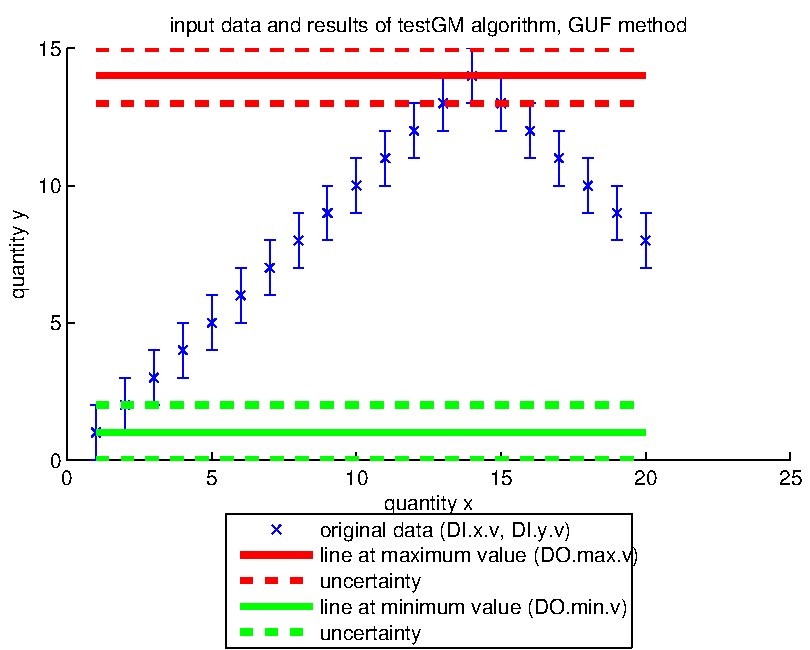
\includegraphics[width=0.7\textwidth]{alg_examples_published/testGM_alg_example_01.pdf}
\end{center}
\begin{par}
Plot histogram of calculated maximal value, i.e. probability density function simulated by Monte Carlo method and overlay by result of GUF method (approximately scaled to MCM result).
\end{par} \vspace{1em}
\begin{lstlisting}[style=mcode]
figure
hold on
hist(DOMCM.max.r, 50)
a = axis;
x = [a(1):0.1:a(2)];
pdf = normpdf(x, DOGUF.max.v, DOGUF.max.u);
plot(x, a(4)/max(pdf).*pdf, '-r', 'linewidth', 4);
title('results of maximum value (DO.max.r)')
legend('Monte Carlo results', 'GUF result (approximately scaled to MCM results', 'location', 'southoutside')
hold off
\end{lstlisting}

\begin{center}
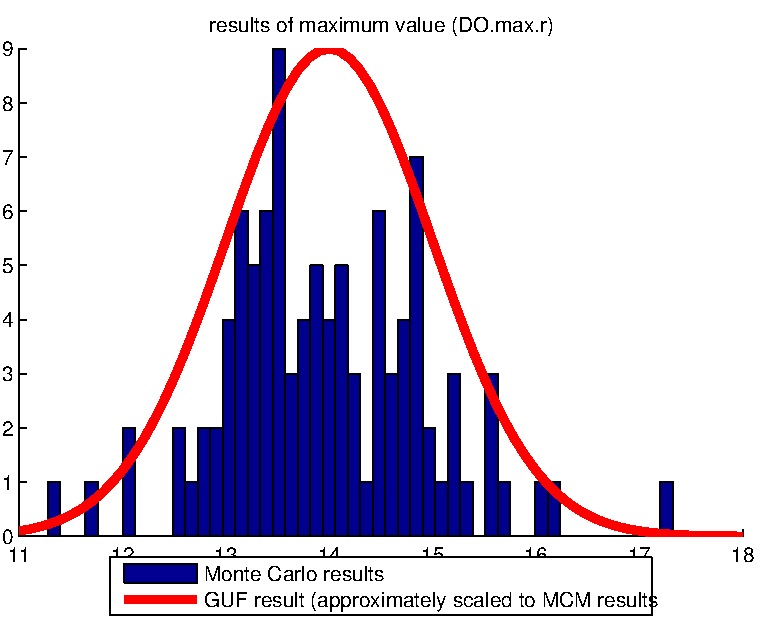
\includegraphics[width=0.7\textwidth]{alg_examples_published/testGM_alg_example_02.pdf}
\end{center}



%%% \end{document}
    

% 
% \chapter{testM -- testM} 
% % included files are automatically generated by info_all_algs.m script and by Matlab publish
% % function and converted by bash script betterpublish.
% \section*{\infosection} 
% \begin{tightdesc}
\item [Id:] testM
\item [Name:] Test with MCM
\item [Description:] Calculates maximum value of the measured record
\item [Citation:] see EMRP Q-Wave
\item [Remarks:] Do not use. This is only for testing QWTB
\item [License:] MIT License
\item [Provides GUF:] no
\item [Provides MCM:] yes
\item [Input Quantities] \rule{0em}{0em}
    \begin{tightdesc}
    \item [Required:] 
        \textsf{x},\enspace \textsf{y}
    \end{tightdesc}
\item [Descriptions:] \rule{0em}{0em}
    \begin{tightdesc}
        \item[\textsf{x}] -- independent quantity
        \item[\textsf{y}] -- dependent quantity
    \end{tightdesc}
\item [Output Quantities] \rule{0em}{0em}
    \begin{tightdesc}
        \item[\textsf{max}] -- maximal dependent quantity
        \item[\textsf{min}] -- minimal dependent quantity
    \end{tightdesc}
\end{tightdesc}

% \section*{\examplesection}
% 
% This LaTeX was auto-generated from an M-file by MATLAB.
% To make changes, update the M-file and republish this document.

%%% \documentclass{article}
%%% \usepackage{graphicx}
%%% \usepackage{color}

%%% \sloppy
%%% \definecolor{lightgray}{gray}{0.5}
\setlength{\parindent}{0pt}

%%% \begin{document}

    
    
\subsection*{testM}

\begin{par}
Example for algorithm testM. Algorithm is usefull only for testing QWTB toolbox. It calculates maximal and minimal value of the record. MCM is calculated by wrapper.
\end{par} \vspace{1em}
\begin{par}
See also \lstinline{qwtb}
\end{par} \vspace{1em}

\subsubsection*{Contents}

\begin{itemize}
\setlength{\itemsep}{-1ex}
   \item Generate sample data
   \item Call algorithm
   \item Plot results
\end{itemize}


\subsubsection*{Generate sample data}

\begin{par}
Two quantities are prepared: \lstinline{x} and \lstinline{y}.
\end{par} \vspace{1em}
\begin{lstlisting}[style=mcode]
x = []; y = [];
x.v = [1:20];
y.v = [1:14 13:-1:8];
\end{lstlisting}
\begin{par}
All uncertainties are set to 1.
\end{par} \vspace{1em}
\begin{lstlisting}[style=mcode]
x.u = x.v.*0 + 1;
y.u = y.v.*0 + 1;
\end{lstlisting}
\begin{par}
Quantities are put into data input structure \lstinline{DI}.
\end{par} \vspace{1em}
\begin{lstlisting}[style=mcode]
DI = [];
DI.x = x;
DI.y = y;
\end{lstlisting}
\begin{par}
Create calculation settings \lstinline{CS} and set uncertainty calculation method to Monte Carlo method. Allow randomization of uncertainties by the QWTB toolbox.
\end{par} \vspace{1em}
\begin{lstlisting}[style=mcode]
CS = [];
CS.unc = 'mcm';
CS.mcm.randomize = 1;
\end{lstlisting}


\subsubsection*{Call algorithm}

\begin{par}
Use QWTB to apply algorithm \lstinline{testM} to data \lstinline{DI} with calculation settings \lstinline{CS}.
\end{par} \vspace{1em}
\begin{lstlisting}[style=mcode]
DO = qwtb('testM', DI, CS);
\end{lstlisting}

        \begin{lstlisting}[style=output]
QWTB: default correlation matrix generated for quantity `x`
QWTB: quantity x was randomized by QWTB
QWTB: default correlation matrix generated for quantity `y`
QWTB: quantity y was randomized by QWTB
QWTB: uncertainty calculation by means of wrapper or algorithm
\end{lstlisting} \color{black}
    

\subsubsection*{Plot results}

\begin{par}
Plot input data and calculated maximal and minimal values as a red and green lines with uncertainties represented by dashed lines.
\end{par} \vspace{1em}
\begin{lstlisting}[style=mcode]
figure
hold on
errorbar(DI.x.v, DI.y.v, DI.y.u, 'xb')
plot([DI.x.v(1) DI.x.v(end)], [DO.max.v DO.max.v], '-r', 'linewidth', 3)
plot([DI.x.v(1) DI.x.v(end)], [DO.max.v - DO.max.u DO.max.v - DO.max.u], '--r', 'linewidth', 3)
plot([DI.x.v(1) DI.x.v(end)], [DO.min.v DO.min.v], '-g', 'linewidth', 3)
plot([DI.x.v(1) DI.x.v(end)], [DO.min.v - DO.min.u DO.min.v - DO.min.u], '--g', 'linewidth', 3)
plot([DI.x.v(1) DI.x.v(end)], [DO.max.v + DO.max.u DO.max.v + DO.max.u], '--r', 'linewidth', 3)
plot([DI.x.v(1) DI.x.v(end)], [DO.min.v + DO.min.u DO.min.v + DO.min.u], '--g', 'linewidth', 3)
legend('original data (DI.x.v, DI.y.v)', 'line at maximum value (DO.max.v)', 'uncertainty',  'line at minimum value (DO.min.v)', 'uncertainty', 'location', 'southoutside')
xlabel('quantity x')
ylabel('quantity y')
title('input data and results of testM algorithm')
hold off
\end{lstlisting}

\begin{center}
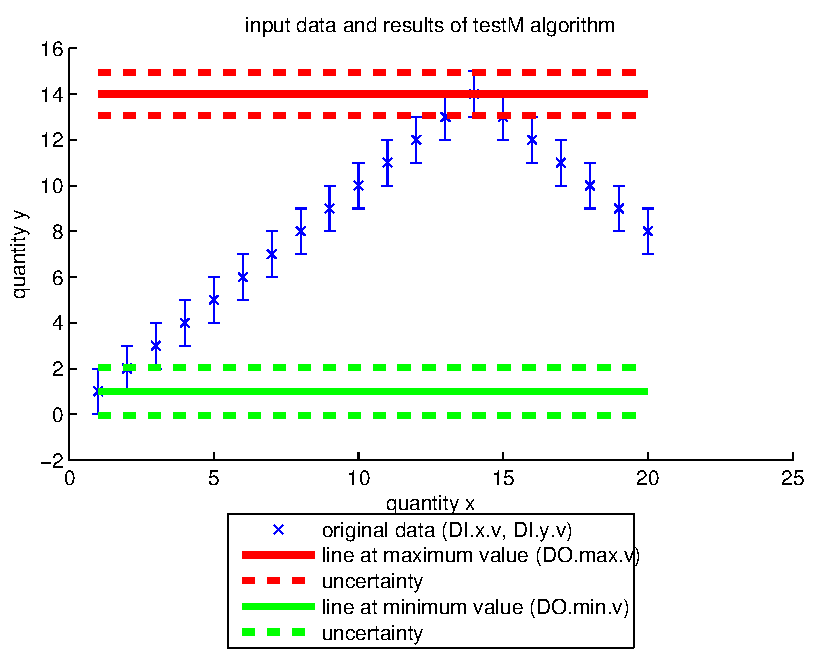
\includegraphics[width=0.7\textwidth]{alg_examples_published/testM_alg_example_01.pdf}
\end{center}
\begin{par}
Plot histogram of calculated maximal value, i.e. probability density function simulated by Monte Carlo method.
\end{par} \vspace{1em}
\begin{lstlisting}[style=mcode]
figure
hist(DO.max.r, 50)
title('histogram of Monte Carlo method results of maximum value (DO.max.r)')
\end{lstlisting}

\begin{center}
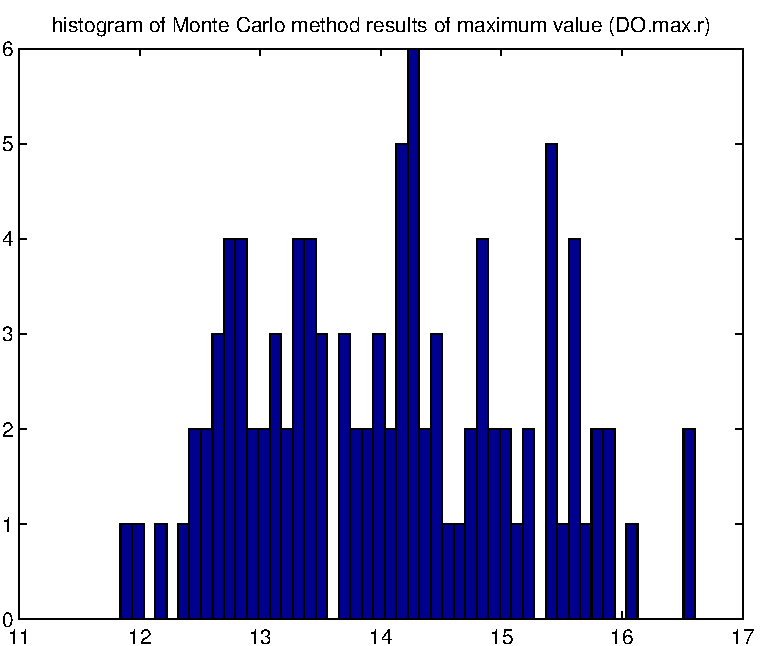
\includegraphics[width=0.7\textwidth]{alg_examples_published/testM_alg_example_02.pdf}
\end{center}



%%% \end{document}
    

% 
% \chapter{testQ -- testQ}
% % included files are automatically generated by info_all_algs.m script and by Matlab publish
% % function and converted by bash script betterpublish.
% \section*{\infosection}
% \begin{tightdesc}
\item [Id:] testQ
\item [Name:] Test of various input Quantities settings
\item [Description:] Calculates minimum and maximum value of |v| quantity, or |u| quantity if present.
\item [Citation:] see EMRP Q-Wave
\item [Remarks:] Do not use. This is only for testing QWTB
\item [License:] MIT License
\item [Provides GUF:] yes
\item [Provides MCM:] no
\item [Input Quantities] \rule{0em}{0em}
    \begin{tightdesc}
    \item [Required:] 
        \textsf{u} or \textsf{v},\enspace \textsf{x} or \textsf{y},\enspace \textsf{a},\enspace \textsf{c}
    \item [Optional:] 
        \textsf{r} or \textsf{s},\enspace \textsf{b},\enspace \textsf{d}
    \item [Parameters:] 
        \textsf{c},\enspace \textsf{d}
    \end{tightdesc}
\item [Descriptions:] \rule{0em}{0em}
    \begin{tightdesc}
        \item[\textsf{a}] -- test a
        \item[\textsf{b}] -- test b
        \item[\textsf{c}] -- test c
        \item[\textsf{d}] -- test d
        \item[\textsf{r}] -- test r
        \item[\textsf{s}] -- test s
        \item[\textsf{u}] -- test u
        \item[\textsf{v}] -- test v
        \item[\textsf{x}] -- test x
        \item[\textsf{y}] -- test y
    \end{tightdesc}
\item [Output Quantities] \rule{0em}{0em}
    \begin{tightdesc}
        \item[\textsf{max}] -- maximal dependent quantity
        \item[\textsf{min}] -- minimal dependent quantity
    \end{tightdesc}
\end{tightdesc}

% \section*{\examplesection}
% %
% This LaTeX was auto-generated from an M-file by MATLAB.
% To make changes, update the M-file and republish this document.

%%% \documentclass{article}
%%% \usepackage{graphicx}
%%% \usepackage{color}

%%% \sloppy
%%% \definecolor{lightgray}{gray}{0.5}
\setlength{\parindent}{0pt}

%%% \begin{document}

    
    
\subsection*{testQ}

\begin{par}
Example for algorithm testQ. Algorithm is usefull only for testing QWTB toolbox. It returns values from the input. This script has no real sense.
\end{par} \vspace{1em}
\begin{par}
See also \lstinline{qwtb}
\end{par} \vspace{1em}

\subsubsection*{Contents}

\begin{itemize}
\setlength{\itemsep}{-1ex}
   \item Generate sample data
   \item Call algorithm
   \item Different input
\end{itemize}


\subsubsection*{Generate sample data}

\begin{par}
Quantities are prepared.
\end{par} \vspace{1em}
\begin{lstlisting}[style=mcode]
DI = [];
DI.x.v = [-5:-1:-1];
DI.v.v = [1:10];
DI.a.v = 5;
DI.c.v = 'variable c';
\end{lstlisting}


\subsubsection*{Call algorithm}

\begin{par}
Use QWTB to apply algorithm \lstinline{testQ} to data \lstinline{DI}.
\end{par} \vspace{1em}
\begin{lstlisting}[style=mcode]
DO = qwtb('testQ', DI);
\end{lstlisting}

        \begin{lstlisting}[style=output]
QWTB: no uncertainty calculation
\end{lstlisting} \color{black}
    \begin{par}
The result is value of \lstinline{v}:
\end{par} \vspace{1em}
\begin{lstlisting}[style=mcode]
DO.e.v
\end{lstlisting}

        \begin{lstlisting}[style=output]

ans =

     []

\end{lstlisting} \color{black}
    

\subsubsection*{Different input}

\begin{par}
Add quantity \lstinline{u}, which has precedence over \lstinline{v}:
\end{par} \vspace{1em}
\begin{lstlisting}[style=mcode]
DI.u.v = [100:110];
DO = qwtb('testQ', DI);
\end{lstlisting}

        \begin{lstlisting}[style=output]
QWTB: no uncertainty calculation
\end{lstlisting} \color{black}
    \begin{par}
The result is value of \lstinline{u}:
\end{par} \vspace{1em}
\begin{lstlisting}[style=mcode]
DO.e.v
\end{lstlisting}

        \begin{lstlisting}[style=output]

ans =

     []

\end{lstlisting} \color{black}
    


%%% \end{document}
    


\chapter{ADEV -- Allan Deviation} %<<<1 ------------------------------
\chaptermark{ADEV}
% included files are automatically generated by info_all_algs.m script and by Matlab publish
% function and converted by bash script betterpublish.
\section*{\infosection} %<<<2 -------------------
\begin{tightdesc}
\item [Id:] ADEV
\item [Name:] Allan Deviation
\item [Description:] Compute the Allan deviation for a set of time-domain frequency data.
\item [Citation:] D.W. Allan, "The Statistics of Atomic Frequency Standards", Proc. IEEE, Vol. 54, No. 2, pp. 221-230, Feb. 1966. Implementation by M. A. Hopcroft, mhopeng@gmail.com, Matlab Central, online: \url{http://www.mathworks.com/matlabcentral/fileexchange/13246-allan} Test data by W. J. Riley, "The Calculation of Time Domain Frequency Stability", online: \url{http://www.wriley.com/paper1ht.htm}
\item [Remarks:] If sampling frequency |fs| is not supplied, wrapper will calculate |fs| from sampling time |Ts| or if not supplied, first two elements of time series |t| are used to calculate |Ts|. If observation time(s) |tau| is not supplied, tau values are automatically generated. Tau values must be divisible by 1/|fs|. Invalid values are ignored. For tau values really used in the calculation see the output.
\item [License:] BSD License
\item [Provides GUF:] yes
\item [Provides MCM:] no
\item [Input Quantities] \rule{0em}{0em}
    \begin{tightdesc}
    \item [Required:] 
        \textsf{fs} or \textsf{Ts} or \textsf{t},\enspace \textsf{y}
    \item [Optional:] 
        \textsf{tau}
    \end{tightdesc}
\item [Descriptions:] \rule{0em}{0em}
    \begin{tightdesc}
        \item[\textsf{Ts}] -- Sampling time
        \item[\textsf{fs}] -- Sampling frequency
        \item[\textsf{t}] -- Time series
        \item[\textsf{tau}] -- Observation time
        \item[\textsf{y}] -- Sampled values
    \end{tightdesc}
\item [Output Quantities] \rule{0em}{0em}
    \begin{tightdesc}
        \item[\textsf{adev}] -- Allan deviation
        \item[\textsf{tau}] -- Observation time of resulted values
    \end{tightdesc}
\end{tightdesc}

\section*{\examplesection} %<<<2 ------------------------

% This LaTeX was auto-generated from an M-file by MATLAB.
% To make changes, update the M-file and republish this document.

%%% \documentclass{article}
%%% \usepackage{graphicx}
%%% \usepackage{color}

%%% \sloppy
%%% \definecolor{lightgray}{gray}{0.5}
\setlength{\parindent}{0pt}

%%% \begin{document}

    
    
\subsection*{Allan Deviation}

\begin{par}
Example for algorithm ADEV.
\end{par} \vspace{1em}
\begin{par}
ADEV is an algorithm to compute the Allan deviation for a set of time-domain frequency data.
\end{par} \vspace{1em}
\begin{par}
See also W. J. Riley, "The Calculation of Time Domain Frequency Stability". Implementation: M. A. Hopcroft, \verb"mhopeng@gmail.com", Matlab Central.'
\end{par} \vspace{1em}

\subsubsection*{Contents}

\begin{itemize}
\setlength{\itemsep}{-1ex}
   \item Generate sample data
   \item Call algorithm
   \item Display results
\end{itemize}


\subsubsection*{Generate sample data}

\begin{lstlisting}[style=mcode]
DI = [];
%!demo
%ysin=2.*sin(2.*pi.*1/300.*[1:1:1e3]);
%! [x y s errors]=adev(1, ysin, 1, 'best averaging time is 300 s, i.e. cca one sine period');
% A random numbers with normal probability distribution function will be geneated into data input |DI.y.v|.
DI.y.v = normrnd(1.5,3,1,1e3);
% Next a drift is added:
DI.y.v = DI.y.v + [1:1:1e3]./100;
% Lets suppose a sampling frequency is 1 Hz:
DI.fs.v = 1;
% Let the algorithm generate all possible tau values automatically:
DI.tau.v = [];
\end{lstlisting}


\subsubsection*{Call algorithm}

\begin{par}
Use QWTB to apply algorithm \lstinline{ADEV} to data \lstinline{DI}.
\end{par} \vspace{1em}
\begin{lstlisting}[style=mcode]
DO = qwtb('ADEV', DI);
\end{lstlisting}

        \begin{lstlisting}[style=output]
QWTB: no uncertainty calculation
\end{lstlisting} \color{black}
    

\subsubsection*{Display results}

\begin{par}
Log log figure is the best to see allan deviation results:
\end{par} \vspace{1em}
\begin{lstlisting}[style=mcode]
figure; hold on
loglog(DO.tau.v, DO.adev.v, '-b')
loglog(DO.tau.v, DO.adev.v + DO.adev.u, '-k')
loglog(DO.tau.v, DO.adev.v - DO.adev.u, '-k')
xlabel('\tau (sec)');
ylabel('\sigma_y(\tau)');
title(['period = ' num2str(DI.fs.v)]);
grid('on'); hold off
\end{lstlisting}

\begin{center}
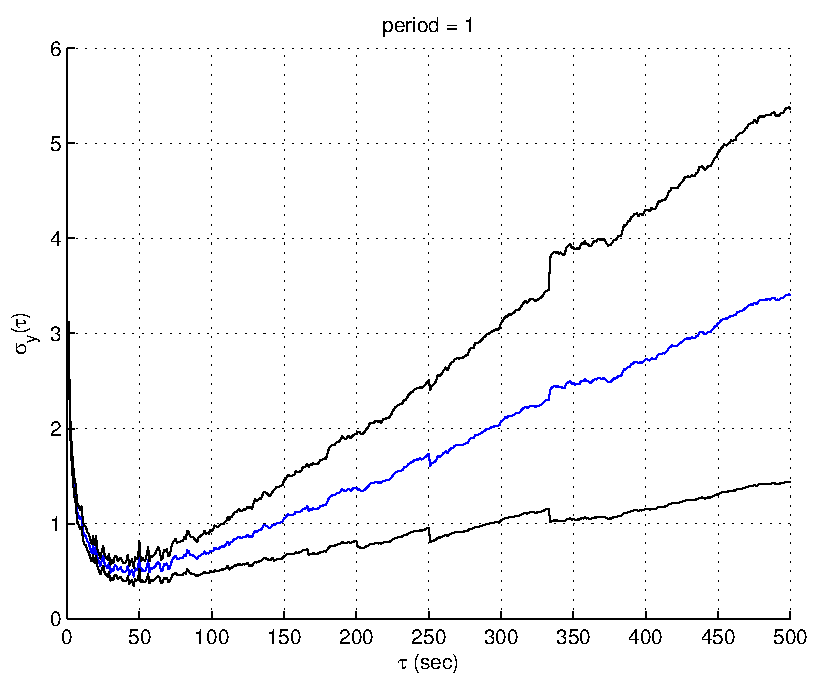
\includegraphics[width=0.7\textwidth]{algs_examples_published/ADEV_alg_example_01.pdf}
\end{center}



%%% \end{document}
    


\chapter{FourPSF -- Standard Four Parameter Sine Wave Fit according IEEE Std 1241-2000} %<<<1 ------------------------------
\chaptermark{FourPSF}
% included files are automatically generated by info_all_algs.m script and by Matlab publish
% function and converted by bash script betterpublish.
\section*{\infosection} %<<<2 -------------------
\begin{tightdesc}
\item [Id:] FourPSF
\item [Name:] Standard Four Parameter Sine Wave Fit according IEEE Std 1241-2000
\item [Description:] Fits a sine wave to the recorded data using 4 parameter (frequency, amplitude, phase and offset) model. The algorithm is according IEEE Standard for Terminology and Test methods for Analog-to-Digital Converters 1241-2000
\item [Citation:] IEEE Std 1241-2000, Implementation written by Zoltán Tamás Bilau, modified by Janos Markus. Id: sfit4.m,v 3.0 2004/04/19 11:20:09 markus Exp. Copyright (c) 2001-2004 by Istvan Kollar and Janos Markus. Modified 2016 Rado Lapuh
\item [Remarks:] If sampling time |Ts| is not supplied, wrapper will calculate |Ts| from sampling frequency |fs| or if not supplied, mean of differences of time series |t| is used to calculate |Ts|.
\item [License:] UNKNOWN
\item [Provides GUF:] no
\item [Provides MCM:] no
\item [Input Quantities] \rule{0em}{0em}
    \begin{tightdesc}
    \item [Required:] 
        \textsf{Ts} or \textsf{fs} or \textsf{t},\enspace \textsf{y}
    \item [Descriptions:] \rule{0em}{0em}
        \begin{tightdesc}
            \item[\textsf{Ts}] -- Sampling time
            \item[\textsf{fs}] -- Sampling frequency
            \item[\textsf{t}] -- Time series
            \item[\textsf{y}] -- Sampled values
        \end{tightdesc}
    \end{tightdesc}
\item [Output Quantities:] \rule{0em}{0em}
    \begin{tightdesc}
        \item[\textsf{A}] -- Amplitude of main signal component
        \item[\textsf{O}] -- Offset of signal
        \item[\textsf{f}] -- Frequency of main signal component
        \item[\textsf{ph}] -- Phase of main signal component
    \end{tightdesc}
\end{tightdesc}

\section*{\examplesection} %<<<2 ------------------------

% This LaTeX was auto-generated from an M-file by MATLAB.
% To make changes, update the M-file and republish this document.

%%% \documentclass{article}
%%% \usepackage{graphicx}
%%% \usepackage{color}

%%% \sloppy
%%% \definecolor{lightgray}{gray}{0.5}
\setlength{\parindent}{0pt}

%%% \begin{document}

    
    
\subsection*{Four parameter sine wave fitting}

\begin{par}
Example for algorithm FourPSF.
\end{par} \vspace{1em}
\begin{par}
FourPSF is an algorithm for estimating the frequency, amplitude, phase and offset of the sine waveform according standard IEEE Std 1241-2000';
\end{par} \vspace{1em}

\subsubsection*{Contents}

\begin{itemize}
\setlength{\itemsep}{-1ex}
   \item Generate sample data
   \item Call algorithm
   \item Display results
\end{itemize}


\subsubsection*{Generate sample data}

\begin{par}
Two quantities are prepared: \lstinline{t} and \lstinline{y}, representing 1 second of sinus waveform of nominal frequency 1 kHz, nominal amplitude 1 V, nominal phase 1 rad and offset 1 V sampled at sampling frequency 10 kHz.
\end{par} \vspace{1em}
\begin{lstlisting}[style=mcode]
DI = [];
Anom = 2; fnom = 100; phnom = 1; Onom = 0.2;
DI.t.v = [0:1/1e4:1-1/1e4];
DI.y.v = Anom*sin(2*pi*fnom*DI.t.v + phnom) + Onom;
\end{lstlisting}


\subsubsection*{Call algorithm}

\begin{par}
Use QWTB to apply algorithm \lstinline{FourPSF} to data \lstinline{DI}.
\end{par} \vspace{1em}
\begin{lstlisting}[style=mcode]
CS.verbose = 1;
DO = qwtb('FourPSF', DI, CS);
\end{lstlisting}

        \begin{lstlisting}[style=output]
QWTB: no uncertainty calculation
QWTB: FourPSF wrapper: sampling time was calculated from time series
\end{lstlisting} \color{black}
    

\subsubsection*{Display results}

\begin{par}
Results is the amplitude, frequency, phase and offset of sampled waveform.
\end{par} \vspace{1em}
\begin{lstlisting}[style=mcode]
A = DO.A.v
f = DO.f.v
ph = DO.ph.v
O = DO.O.v
\end{lstlisting}

        \begin{lstlisting}[style=output]

A =

    2.0000


f =

   100


ph =

    1.0000


O =

    0.2000

\end{lstlisting} \color{black}
    \begin{par}
Errors of estimation in parts per milion:
\end{par} \vspace{1em}
\begin{lstlisting}[style=mcode]
Aerrppm = (DO.A.v - Anom)/Anom .* 1e6
ferrppm = (DO.f.v - fnom)/fnom .* 1e6
pherrppm = (DO.ph.v - phnom)/phnom .* 1e6
Oerrppm = (DO.O.v - Onom)/Onom .* 1e6
\end{lstlisting}

        \begin{lstlisting}[style=output]

Aerrppm =

   2.2204e-09


ferrppm =

     0


pherrppm =

   8.8818e-09


Oerrppm =

   1.3878e-09

\end{lstlisting} \color{black}
    


%%% \end{document}
    


\chapter{FPNLSF -- Four Parameter Non-Linear Sine Fit} %<<<1 ------------------------------
\chaptermark{FPNLSF}
% included files are automatically generated by info_all_algs.m script and by Matlab publish
% function and converted by bash script betterpublish.
\section*{\infosection} %<<<2 -------------------
\begin{tightdesc}
\item [Id:] FPNLSF
\item [Name:] Four Parameter Non-Linear Sine Fit
\item [Description:] Fits a sine wave to the recorded data by means of non-linear least squares fitting method using 4 parameter (frequency, amplitude, phase and offset) model. An estimate of signal frequency is required. Due to non-linear characteristic, convergence is not always achieved. When run in Matlab, function `lsqnonlin` in Optimization toolbox is used. When run in GNU Octave, function `leasqr` in GNU Octave Forge package optim is used. Therefore results can differ.
\item [Citation:] 
\item [Remarks:] If Time series |t| is not supplied, wrapper will calculate |t| from sampling frequency |fs| or if not supplied, sampling time |Ts| is used to calculate |t|.
\item [License:] MIT License
\item [Provides GUF:] no
\item [Provides MCM:] no
\item [Input Quantities] \rule{0em}{0em}
    \begin{tightdesc}
    \item [Required:] 
        \textsf{t} or \textsf{fs} or \textsf{Ts},\enspace \textsf{y},\enspace \textsf{fest}
    \item [Descriptions:] \rule{0em}{0em}
        \begin{tightdesc}
            \item[\textsf{Ts}] -- Sampling time
            \item[\textsf{fest}] -- Estimate of signal frequency
            \item[\textsf{fs}] -- Sampling frequency
            \item[\textsf{t}] -- Time series
            \item[\textsf{y}] -- Sampled values
        \end{tightdesc}
    \end{tightdesc}
\item [Output Quantities:] \rule{0em}{0em}
    \begin{tightdesc}
        \item[\textsf{A}] -- Amplitude of main signal component
        \item[\textsf{O}] -- Offset of signal
        \item[\textsf{f}] -- Frequency of main signal component
        \item[\textsf{ph}] -- Phase of main signal component
    \end{tightdesc}
\end{tightdesc}

\section*{\examplesection} %<<<2 ------------------------

% This LaTeX was auto-generated from an M-file by MATLAB.
% To make changes, update the M-file and republish this document.

%%% \documentclass{article}
%%% \usepackage{graphicx}
%%% \usepackage{color}

%%% \sloppy
%%% \definecolor{lightgray}{gray}{0.5}
\setlength{\parindent}{0pt}

%%% \begin{document}

    
    
\subsection*{Four parameter sine wave fitting}

\begin{par}
Example for algorithm FPNLSF.
\end{par} \vspace{1em}
\begin{par}
FPNLSF is an algorithm for estimating the frequency, amplitude, and phase of the sine waveform. The algorithm use least squares method. Algorithm requires good estimate of frequency.
\end{par} \vspace{1em}

\subsubsection*{Contents}

\begin{itemize}
\setlength{\itemsep}{-1ex}
   \item Generate sample data
   \item Call algorithm
   \item Display results
\end{itemize}


\subsubsection*{Generate sample data}

\begin{par}
Two quantities are prepared: \lstinline{t} and \lstinline{y}, representing 1 second of sinus waveform of nominal frequency 1 kHz, nominal amplitude 1 V, nominal phase 1 rad and offset 1 V sampled at sampling frequency 10 kHz.
\end{par} \vspace{1em}
\begin{lstlisting}[style=mcode]
DI = [];
Anom = 2; fnom = 100; phnom = 1; Onom = 0.2;
DI.t.v = [0:1/1e4:1-1/1e4];
DI.y.v = Anom*sin(2*pi*fnom*DI.t.v + phnom) + Onom;
\end{lstlisting}
\begin{par}
Lets make an estimate of frequency 0.2 percent higher than nominal value:
\end{par} \vspace{1em}
\begin{lstlisting}[style=mcode]
DI.fest.v = 100.2;
\end{lstlisting}


\subsubsection*{Call algorithm}

\begin{par}
Use QWTB to apply algorithm \lstinline{FPNLSF} to data \lstinline{DI}.
\end{par} \vspace{1em}
\begin{lstlisting}[style=mcode]
CS.verbose = 1;
DO = qwtb('FPNLSF', DI, CS);
\end{lstlisting}

        \begin{lstlisting}[style=output]
QWTB: no uncertainty calculation
Fitting started

Local minimum found.

Optimization completed because the size of the gradient is less than
the default value of the function tolerance.



Fitting finished
\end{lstlisting} \color{black}
    

\subsubsection*{Display results}

\begin{par}
Results is the amplitude, frequency and phase of sampled waveform.
\end{par} \vspace{1em}
\begin{lstlisting}[style=mcode]
A = DO.A.v
f = DO.f.v
ph = DO.ph.v
O = DO.O.v
\end{lstlisting}

        \begin{lstlisting}[style=output]

A =

    2.0000


f =

   100


ph =

    1.0000


O =

    0.2000

\end{lstlisting} \color{black}
    \begin{par}
Errors of estimation in parts per milion:
\end{par} \vspace{1em}
\begin{lstlisting}[style=mcode]
Aerrppm = (DO.A.v - Anom)/Anom .* 1e6
ferrppm = (DO.f.v - fnom)/fnom .* 1e6
pherrppm = (DO.ph.v - phnom)/phnom .* 1e6
Oerrppm = (DO.O.v - Onom)/Onom .* 1e6
\end{lstlisting}

        \begin{lstlisting}[style=output]

Aerrppm =

   4.8894e-07


ferrppm =

     0


pherrppm =

   4.8850e-09


Oerrppm =

  -1.1102e-08

\end{lstlisting} \color{black}
    


%%% \end{document}
    


\chapter{iDFT2p -- 2-point interpolated DFT frequency estimator} %<<<1 ------------------------------
\chaptermark{iDFT2p}
% included files are automatically generated by info_all_algs.m script and by Matlab publish
% function and converted by bash script betterpublish.
\section*{\infosection} %<<<2 -------------------
\begin{tightdesc}
\item [Id:] iDFT2p
\item [Name:] 2-point interpolated DFT frequency estimator
\item [Description:] An algorithm for estimating the frequency, amplitude, phase and offset of the fundamental component using interpolated discrete Fourier transform. Rectangular or Hann window can be used for DFT.
\item [Citation:] Krzysztof Duda: Interpolation algorithms of DFT for parameters estimation of sinusoidal and damped sinusoidal signals. In S. M. Salih, editor, Fourier Transform - Signal Processing, chapter 1, pages 3-32, InTech, 2012. \url{http://www.intechopen.com/books/fourier-transform-signal-processing/interpolated-dft} Implemented by Rado Lapuh, 2016.
\item [Remarks:] If sampling time |Ts| is not supplied, wrapper will calculate |Ts| from sampling frequency |fs| or if not supplied, mean of differences of time series |t| is used to calculate |Ts|. The optional parameter |window| can be set to values `rectangular` or `Hann`. If parameter is not supplied, Hann window will be used.
\item [License:] Implementation: MIT License
\item [Provides GUF:] no
\item [Provides MCM:] no
\item [Input Quantities] \rule{0em}{0em}
    \begin{tightdesc}
    \item [Required:] 
        \textsf{Ts} or \textsf{fs} or \textsf{t},\enspace \textsf{y}
    \item [Optional:] 
        \textsf{window}
    \item [Parameters:] 
        \textsf{window}
    \item [Descriptions:] \rule{0em}{0em}
        \begin{tightdesc}
            \item[\textsf{Ts}] -- Sampling time
            \item[\textsf{fs}] -- Sampling frequency
            \item[\textsf{t}] -- Time series
            \item[\textsf{window}] -- DFT window: `Hann` or `rectangular`
            \item[\textsf{y}] -- Sampled values
        \end{tightdesc}
    \end{tightdesc}
\item [Output Quantities:] \rule{0em}{0em}
    \begin{tightdesc}
        \item[\textsf{A}] -- Amplitude of main signal component
        \item[\textsf{O}] -- Offset of main signal component
        \item[\textsf{f}] -- Frequency of main signal component
        \item[\textsf{ph}] -- Phase of main signal component
    \end{tightdesc}
\end{tightdesc}

\section*{\examplesection} %<<<2 ------------------------

% This LaTeX was auto-generated from an M-file by MATLAB.
% To make changes, update the M-file and republish this document.

%%% \documentclass{article}
%%% \usepackage{graphicx}
%%% \usepackage{color}

%%% \sloppy
%%% \definecolor{lightgray}{gray}{0.5}
\setlength{\parindent}{0pt}

%%% \begin{document}

    
    
\subsection*{2-point interpolated DFT frequency estimator}

\begin{par}
Example for algorithm iDFT3p.
\end{par} \vspace{1em}
\begin{par}
iDFT2p is an algorithm for estimating the frequency, amplitude, and phase of the fundamental component using interpolated discrete Fourier transform. Rectangular or Hann window can be used for DFT.'; See also Krzysztof Duda: Interpolation algorithms of DFT for parameters estimation of sinusoidal and damped sinusoidal signals. In S. M. Salih, editor, Fourier Transform - Signal Processing, chapter 1, pages 3-32, InTech, 2012. \url{http://www.intechopen.com/books/fourier-transform-signal-processing/interpolated-dft} Implemented by Rado Lapuh, 2016.';
\end{par} \vspace{1em}

\subsubsection*{Contents}

\begin{itemize}
\setlength{\itemsep}{-1ex}
   \item Generate sample data
   \item Call algorithm
   \item Display results
\end{itemize}


\subsubsection*{Generate sample data}

\begin{par}
Two quantities are prepared: \lstinline{Ts} and \lstinline{y}, representing 0.5 second of sinus waveform of nominal frequency 100 Hz, nominal amplitude 1 V and nominal phase 1 rad, sampled with sampling time 0.1 ms, with offset 0.1 V. The sampling is not coherent.
\end{par} \vspace{1em}
\begin{lstlisting}[style=mcode]
DI = [];
Anom = 1; fnom = 100; phnom = 1; Onom = 0.1;
DI.Ts.v = 1e-4;
t = [0:DI.Ts.v:0.5];
DI.y.v = Anom*sin(2*pi*fnom*t + phnom) + Onom;
\end{lstlisting}


\subsubsection*{Call algorithm}

\begin{par}
First a rectangular window will be selected to estimate main signal properties. Use QWTB to apply algorithm \lstinline{iDFT3p} to data \lstinline{DI} and put results into \lstinline{DOr}.
\end{par} \vspace{1em}
\begin{lstlisting}[style=mcode]
DI.window.v = 'rectangular';
DOr = qwtb('iDFT2p', DI);
\end{lstlisting}

        \begin{lstlisting}[style=output]
QWTB: no uncertainty calculation
\end{lstlisting} \color{black}
    \begin{par}
Next a Hann window will be selected to estimate main signal properties Results will be put into \lstinline{DOh}.
\end{par} \vspace{1em}
\begin{lstlisting}[style=mcode]
DI.window.v = 'Hann';
DOh = qwtb('iDFT2p', DI);
\end{lstlisting}

        \begin{lstlisting}[style=output]
QWTB: no uncertainty calculation
\end{lstlisting} \color{black}
    

\subsubsection*{Display results}

\begin{par}
Results is the amplitude, frequency and phase of sampled waveform. For rectangular window, the error from nominal in parts per milion is:
\end{par} \vspace{1em}
\begin{lstlisting}[style=mcode]
f_re = (DOr.f.v - fnom)./fnom .* 1e6
A_re = (DOr.A.v - Anom)./Anom .* 1e6
ph_re = (DOr.ph.v - phnom)./phnom .* 1e6
O_re = (DOr.O.v - Onom)./Onom .* 1e6
\end{lstlisting}

        \begin{lstlisting}[style=output]

f_re =

   -0.8083


A_re =

   40.3148


ph_re =

  217.9412


O_re =

   1.6826e+03

\end{lstlisting} \color{black}
    \begin{par}
For Hann window:
\end{par} \vspace{1em}
\begin{lstlisting}[style=mcode]
f_he = (DOh.f.v - fnom)./fnom .* 1e6
A_he = (DOh.A.v - Anom)./Anom .* 1e6
ph_he = (DOh.ph.v - phnom)./phnom .* 1e6
O_he = (DOh.O.v - Onom)./Onom .* 1e6
\end{lstlisting}

        \begin{lstlisting}[style=output]

f_he =

   1.8426e-04


A_he =

   -0.0046


ph_he =

    6.2442


O_he =

   -0.6862

\end{lstlisting} \color{black}
    


%%% \end{document}
    


\chapter{iDFT3p -- 3-point interpolated DFT frequency estimator} %<<<1 ------------------------------
\chaptermark{iDFT3p}
% included files are automatically generated by info_all_algs.m script and by Matlab publish
% function and converted by bash script betterpublish.
\section*{\infosection} %<<<2 -------------------
\begin{tightdesc}
\item [Id:] iDFT3p
\item [Name:] 3-point interpolated DFT frequency estimator
\item [Description:] An algorithm for estimating the frequency, amplitude, phase and offset of the fundamental component using interpolated discrete Fourier transform. Rectangular or Hann window can be used for DFT.
\item [Citation:] Krzysztof Duda: Interpolation algorithms of DFT for parameters estimation of sinusoidal and damped sinusoidal signals. In S. M. Salih, editor, Fourier Transform - Signal Processing, chapter 1, pages 3-32, InTech, 2012. \url{http://www.intechopen.com/books/fourier-transform-signal-processing/interpolated-dft} Implemented by Rado Lapuh, 2016.
\item [Remarks:] If sampling time |Ts| is not supplied, wrapper will calculate |Ts| from sampling frequency |fs| or if not supplied, mean of differences of time series |t| is used to calculate |Ts|. The optional parameter |window| can be set to values `rectangular` or `Hann`. If parameter is not supplied, Hann window will be used.
\item [License:] Implementation: MIT License
\item [Provides GUF:] no
\item [Provides MCM:] no
\item [Input Quantities] \rule{0em}{0em}
    \begin{tightdesc}
    \item [Required:] 
        \textsf{Ts} or \textsf{fs} or \textsf{t},\enspace \textsf{y}
    \item [Optional:] 
        \textsf{window}
    \item [Parameters:] 
        \textsf{window}
    \item [Descriptions:] \rule{0em}{0em}
        \begin{tightdesc}
            \item[\textsf{Ts}] -- Sampling time
            \item[\textsf{fs}] -- Sampling frequency
            \item[\textsf{t}] -- Time series
            \item[\textsf{window}] -- DFT window: `Hann` or `rectangular`
            \item[\textsf{y}] -- Sampled values
        \end{tightdesc}
    \end{tightdesc}
\item [Output Quantities:] \rule{0em}{0em}
    \begin{tightdesc}
        \item[\textsf{A}] -- Amplitude of main signal component
        \item[\textsf{O}] -- Offset of main signal component
        \item[\textsf{f}] -- Frequency of main signal component
        \item[\textsf{ph}] -- Phase of main signal component
    \end{tightdesc}
\end{tightdesc}

\section*{\examplesection} %<<<2 ------------------------

% This LaTeX was auto-generated from an M-file by MATLAB.
% To make changes, update the M-file and republish this document.

%%% \documentclass{article}
%%% \usepackage{graphicx}
%%% \usepackage{color}

%%% \sloppy
%%% \definecolor{lightgray}{gray}{0.5}
\setlength{\parindent}{0pt}

%%% \begin{document}

    
    
\subsection*{3-point interpolated DFT frequency estimator}

\begin{par}
Example for algorithm iDFT3p.
\end{par} \vspace{1em}
\begin{par}
iDFT3p is an algorithm for estimating the frequency, amplitude, phase and offset of the fundamental component using interpolated discrete Fourier transform. Rectangular or Hann window can be used for DFT.'; See also Krzysztof Duda: Interpolation algorithms of DFT for parameters estimation of sinusoidal and damped sinusoidal signals. In S. M. Salih, editor, Fourier Transform - Signal Processing, chapter 1, pages 3-32, InTech, 2012. \url{http://www.intechopen.com/books/fourier-transform-signal-processing/interpolated-dft} Implemented by Rado Lapuh, 2016.';
\end{par} \vspace{1em}

\subsubsection*{Contents}

\begin{itemize}
\setlength{\itemsep}{-1ex}
   \item Generate sample data
   \item Call algorithm
   \item Display results
\end{itemize}


\subsubsection*{Generate sample data}

\begin{par}
Two quantities are prepared: \lstinline{Ts} and \lstinline{y}, representing 0.5 second of sinus waveform of nominal frequency 100 Hz, nominal amplitude 1 V and nominal phase 1 rad, sampled with sampling time 0.1 ms, with offset 0.1 V. The sampling is not coherent.
\end{par} \vspace{1em}
\begin{lstlisting}[style=mcode]
DI = [];
Anom = 1; fnom = 100; phnom = 1; Onom = 0.1;
DI.Ts.v = 1e-4;
t = [0:DI.Ts.v:0.5];
DI.y.v = Anom*sin(2*pi*fnom*t + phnom) + Onom;
\end{lstlisting}


\subsubsection*{Call algorithm}

\begin{par}
First a rectangular window will be selected to estimate main signal properties. Use QWTB to apply algorithm \lstinline{iDFT3p} to data \lstinline{DI} and put results into \lstinline{DOr}.
\end{par} \vspace{1em}
\begin{lstlisting}[style=mcode]
DI.window.v = 'rectangular';
DOr = qwtb('iDFT3p', DI);
\end{lstlisting}

        \begin{lstlisting}[style=output]
QWTB: no uncertainty calculation
\end{lstlisting} \color{black}
    \begin{par}
Next a Hann window will be selected to estimate main signal properties Results will be put into \lstinline{DOh}.
\end{par} \vspace{1em}
\begin{lstlisting}[style=mcode]
DI.window.v = 'Hann';
DOh = qwtb('iDFT3p', DI);
\end{lstlisting}

        \begin{lstlisting}[style=output]
QWTB: no uncertainty calculation
\end{lstlisting} \color{black}
    

\subsubsection*{Display results}

\begin{par}
Results is the amplitude, frequency and phase of sampled waveform. For rectangular window, the error from nominal in parts per milion is:
\end{par} \vspace{1em}
\begin{lstlisting}[style=mcode]
f_re = (DOr.f.v - fnom)./fnom .* 1e6
A_re = (DOr.A.v - Anom)./Anom .* 1e6
ph_re = (DOr.ph.v - phnom)./phnom .* 1e6
O_re = (DOr.O.v - Onom)./Onom .* 1e6
\end{lstlisting}

        \begin{lstlisting}[style=output]

f_re =

    0.0166


A_re =

   41.2567


ph_re =

   88.3681


O_re =

   1.6826e+03

\end{lstlisting} \color{black}
    \begin{par}
For Hann window:
\end{par} \vspace{1em}
\begin{lstlisting}[style=mcode]
f_he = (DOh.f.v - fnom)./fnom .* 1e6
A_he = (DOh.A.v - Anom)./Anom .* 1e6
ph_he = (DOh.ph.v - phnom)./phnom .* 1e6
O_he = (DOh.O.v - Onom)./Onom .* 1e6
\end{lstlisting}

        \begin{lstlisting}[style=output]

f_he =

  -3.7790e-06


A_he =

   3.9679e-07


ph_he =

    6.2737


O_he =

   -0.6862

\end{lstlisting} \color{black}
    


%%% \end{document}
    


\chapter{INL-DNL -- Integral and Differential Non-Linearity of ADC} %<<<1 ------------------------------
\chaptermark{INL-DNL}
% included files are automatically generated by info_all_algs.m script and by Matlab publish
% function and converted by bash script betterpublish.
\section*{\infosection} %<<<2 -------------------
\begin{tightdesc}
\item [\textsf{.id}] --- INL-DNL
\item [\textsf{.name}] --- Integral and Differential Non-Linearity of ADC
\item [\textsf{.desc}] --- Calculates Integral and Differential Non-Linearity of an ADC. The histogram of measured data is used to calculate INL and DNL estimators. ADC has to sample a pure sine wave. To estimate all transition levels the amplitude of the sine wave should overdrive the full range of the ADC by at least 120%. If not so, non estimated transition levels will be assumed to be 0 and the results may be less accurate. As an input ADC codes are required.
\item [\textsf{.citation}] --- Estimators are based on Tamás Virosztek, MATLAB-based ADC testing with sinusoidal excitation signal (in Hungar- ian), B.Sc. Thesis, 2011. Implementation: Virosztek, T., Pálfi V., Renczes B., Kollár I., Balogh L., Sárhegyi A., Márkus J., Bilau Z. T., ADCTest project site: \url{http://www.mit.bme.hu/projects/adctest} 2000-2014
\item [\textsf{.remarks}] --- Based on the ADCTest Toolbox v4.3, November 25, 2014.
\item [\textsf{.license}] --- UNKNOWN
\item [\textsf{.requires}] \rule{0em}{0em}
\begin{tightdesc}
\item [\textsf{bitres}] --- Bit resolution of the ADC
\item [\textsf{codes}] --- Sampled values represented as ADC codes (not converted to voltage)
\end{tightdesc}
\item [\textsf{.returns}] \rule{0em}{0em}
\begin{tightdesc}
\item [\textsf{DNL}] --- Differential Non-Linearity
\end{tightdesc}
\item [\textsf{.providesGUF}] --- no
\item [\textsf{.providesMCM}] ---  no
\end{tightdesc}

\section*{\examplesection} %<<<2 ------------------------

% This LaTeX was auto-generated from an M-file by MATLAB.
% To make changes, update the M-file and republish this document.

%%% \documentclass{article}
%%% \usepackage{graphicx}
%%% \usepackage{color}

%%% \sloppy
%%% \definecolor{lightgray}{gray}{0.5}
\setlength{\parindent}{0pt}

%%% \begin{document}

    
    
\subsection*{Integral and Differential Non Linearity of ADC}

\begin{par}
Example for algorithm INL-DNL
\end{par} \vspace{1em}
\begin{par}
INL-DNL is an algorithm for estimating Integral and Differential Non-Linearity of an ADC. ADC has to sample a pure sine wave. To estimate all transition levels the amplitude of the sine wave should overdrive the full range of the ADC by at least 120\%. If not so, non estimated transition levels will be assumed to be 0 and the results may be less accurate. As an input ADC codes are required.';
\end{par} \vspace{1em}
\begin{par}
See also 'Virosztek, T., Pálfi V., Renczes B., Kollár I., Balogh L., Sárhegyi A., Márkus J., Bilau Z. T., ADCTest project site: \url{http://www.mit.bme.hu/projects/adctest} 2000-2014';
\end{par} \vspace{1em}

\subsubsection*{Contents}

\begin{itemize}
\setlength{\itemsep}{-1ex}
   \item Generate sample data
   \item Call algorithm
\end{itemize}


\subsubsection*{Generate sample data}

\begin{par}
Suppose a sine wave of nominal frequency 10 Hz and nominal amplitude 1.5 V is sampled by ADC with bit resolution of 4 and full range of 1 V. First quantity \lstinline{bitres} with number of bits of resolution of the ADC is prepared and put into input data structure \lstinline{DI}.
\end{par} \vspace{1em}
\begin{lstlisting}[style=mcode]
DI = [];
DI.bitres.v = 4;
\end{lstlisting}
\begin{par}
Waveform is constructed. Amplitude is selected to overload the ADC.
\end{par} \vspace{1em}
\begin{lstlisting}[style=mcode]
t=[0:1/1e4:1-1/1e4];
Anom = 3.5; fnom = 2; phnom = 0;
wvfrm = Anom*sin(2*pi*fnom*t + phnom);
\end{lstlisting}
\begin{par}
Next ADC code values are calculated. It is simulated by quantization and scaling of the sampled waveform. In real measurement code values can be obtained directly from the ADC. Suppose ADC range is -2..2.
\end{par} \vspace{1em}
\begin{lstlisting}[style=mcode]
codes = wvfrm;
rmin = -2; rmax = 2;
levels = 2.^DI.bitres.v - 1;
codes(codes<rmin) = rmin;
codes(codes>rmax) = rmax;
codes = round((codes-rmin)./(rmax-rmin).*levels);
\end{lstlisting}
\begin{par}
Now lets introduce ADC error. Instead of generating code 2 ADC erroneously generates code 3 and instead of 11 it generates 10.
\end{par} \vspace{1em}
\begin{lstlisting}[style=mcode]
codes(codes==2) = 3;
codes(codes==11) = 10;
codes = codes + min(codes);
\end{lstlisting}
\begin{par}
Create quantity \lstinline{codes} and plot a figure with sampled sine wave and codes.
\end{par} \vspace{1em}
\begin{lstlisting}[style=mcode]
DI.codes.v = codes;
figure
hold on
stairs(t, codes);
wvfrm = (wvfrm - rmin)./(rmax-rmin).*levels;
plot(t, wvfrm, '-r');
xlabel('t (s)')
ylabel('Codes / Voltage (scaled)');
legend('Codes generated by ADC','Original waveform scaled to match codes');
hold off
\end{lstlisting}

\begin{center}
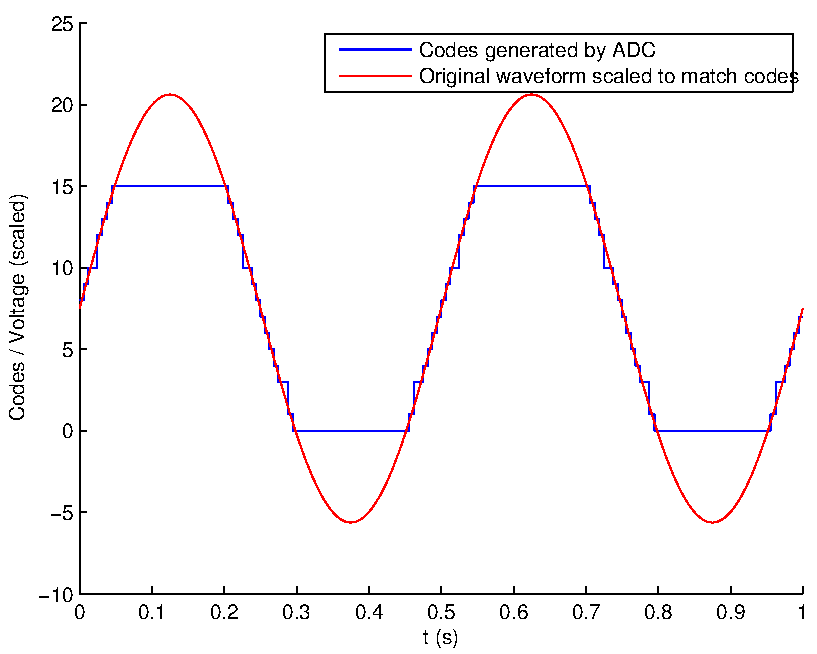
\includegraphics[width=0.7\textwidth]{algs_examples_published/INL-DNL_alg_example_01.pdf}
\end{center}


\subsubsection*{Call algorithm}

\begin{par}
Apply INL algorithm to the input data \lstinline{DI}.
\end{par} \vspace{1em}
\begin{lstlisting}[style=mcode]
DO = qwtb('INL-DNL', DI);
\end{lstlisting}

        \begin{lstlisting}[style=output]
QWTB: no uncertainty calculation
\end{lstlisting} \color{black}
    \begin{par}
Plot results of integral non-linearity. One can clearly observe defects on codes 3 and 11.
\end{par} \vspace{1em}
\begin{lstlisting}[style=mcode]
figure
plot(DO.INL.v, '-x');
xlabel('Transition levels')
ylabel('INL (k)')
% Plot results of differential non-linearity. One can clearly observe defects on transitions 2-3 and
% 10-11.
figure
plot(DO.DNL.v, '-x');
xlabel('Code bins')
ylabel('DNL (k)')
\end{lstlisting}

\begin{center}
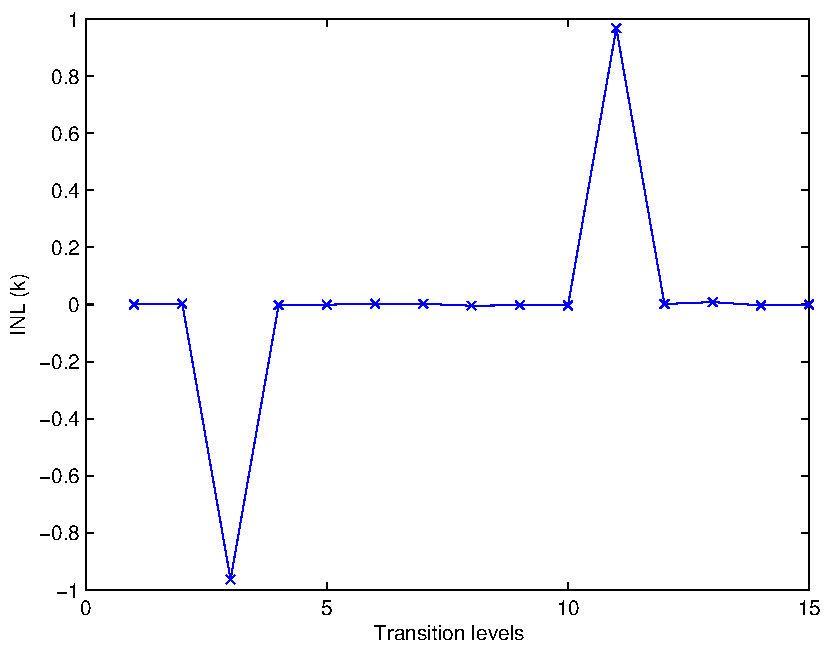
\includegraphics[width=0.7\textwidth]{algs_examples_published/INL-DNL_alg_example_02.pdf}
\end{center}

\begin{center}
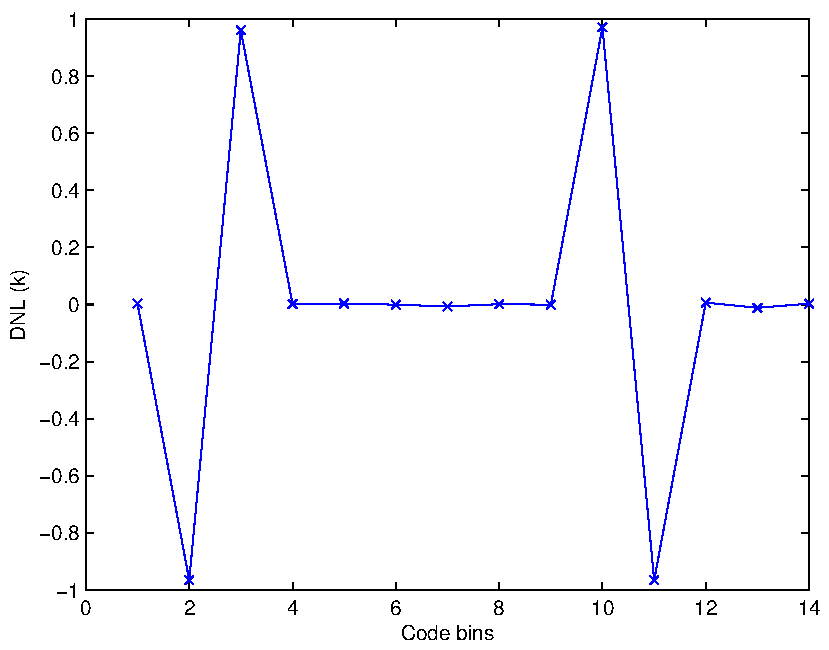
\includegraphics[width=0.7\textwidth]{algs_examples_published/INL-DNL_alg_example_03.pdf}
\end{center}



%%% \end{document}
    


\chapter{MADEV -- Modified Allan Deviation} %<<<1 ------------------------------
\chaptermark{MADEV}
% included files are automatically generated by info_all_algs.m script and by Matlab publish
% function and converted by bash script betterpublish.
\section*{\infosection} %<<<2 -------------------
\begin{tightdesc}
\item [\textsf{.id}] --- MADEV
\item [\textsf{.name}] --- Modified Allan Deviation
\item [\textsf{.desc}] --- Compute the modified Allan deviation for a set of time-domain frequency data.
\item [\textsf{.citation}] --- D.W. Allan and J.A. Barnes, "A Modified Allan Variance with Increased Oscillator Characterization Ability", Proc. 35th Annu. Symp. on Freq. Contrl., pp. 470-474, May 1981. Implementation: Implementation by M. A. Hopcroft, mhopeng@gmail.com, Matlab Central, online: \url{http://www.mathworks.com/matlabcentral/fileexchange/26637-allan-modified} Test data by W. J. Riley, "The Calculation of Time Domain Frequency Stability", online: \url{http://www.wriley.com/paper1ht.htm}
\item [\textsf{.remarks}] --- If tau is empty array, tau values are automatically generated. Tau values must be divisible by 1/fs. Invalid values are ignored. For tau values really used in the calculation see the output. Using sigma as uncertainty is probably not correct.
\item [\textsf{.license}] --- BSD License
\item [\textsf{.requires}] \rule{0em}{0em}
\begin{tightdesc}
\item [\textsf{y}] --- sampled values
\item [\textsf{fs}] --- sampling frequency
\item [\textsf{tau}] --- observation time
\end{tightdesc}
\item [\textsf{.returns}] \rule{0em}{0em}
\begin{tightdesc}
\item [\textsf{madev}] --- modified Allan deviation
\item [\textsf{tau}] --- observation time of result values
\end{tightdesc}
\item [\textsf{.providesGUF}] --- yes
\item [\textsf{.providesMCM}] ---  no
\end{tightdesc}

\section*{\examplesection} %<<<2 ------------------------

% This LaTeX was auto-generated from an M-file by MATLAB.
% To make changes, update the M-file and republish this document.

%%% \documentclass{article}
%%% \usepackage{graphicx}
%%% \usepackage{color}

%%% \sloppy
%%% \definecolor{lightgray}{gray}{0.5}
\setlength{\parindent}{0pt}

%%% \begin{document}

    
    
\subsection*{Modified Allan Deviation}

\begin{par}
Example for algorithm MADEV.
\end{par} \vspace{1em}
\begin{par}
MADEV is an algorithm to compute the modified Allan deviation for a set of time-domain frequency data.
\end{par} \vspace{1em}
\begin{par}
See also W. J. Riley, "The Calculation of Time Domain Frequency Stability". Implementation: M. A. Hopcroft, \verb"mhopeng@gmail.com", Matlab Central.'
\end{par} \vspace{1em}

\subsubsection*{Contents}

\begin{itemize}
\setlength{\itemsep}{-1ex}
   \item Generate sample data
   \item Call algorithm
   \item Display results
\end{itemize}


\subsubsection*{Generate sample data}

\begin{lstlisting}[style=mcode]
DI = [];
%!demo
%ysin=2.*sin(2.*pi.*1/300.*[1:1:1e3]);
%! [x y s errors]=madev(1, ysin, 1, 'best averaging time is 300 s, i.e. cca one sine period');
% A random numbers with normal probability distribution function will be geneated into data input |DI.y.v|.
DI.y.v = normrnd(1.5,3,1,1e3);
% Next a drift is added:
DI.y.v = DI.y.v + [1:1:1e3]./100;
% Lets suppose a sampling frequency is 1 Hz:
DI.fs.v = 1;
% Let the algorithm generate all possible tau values automatically:
DI.tau.v = [];
\end{lstlisting}


\subsubsection*{Call algorithm}

\begin{par}
Use QWTB to apply algorithm \lstinline{MADEV} to data \lstinline{DI}.
\end{par} \vspace{1em}
\begin{lstlisting}[style=mcode]
DO = qwtb('MADEV', DI);
\end{lstlisting}

        \begin{lstlisting}[style=output]
QWTB: no uncertainty calculation
\end{lstlisting} \color{black}
    

\subsubsection*{Display results}

\begin{par}
Log log figure is the best to see modified allan deviation results:
\end{par} \vspace{1em}
\begin{lstlisting}[style=mcode]
figure; hold on
loglog(DO.tau.v, DO.madev.v, '-b')
loglog(DO.tau.v, DO.madev.v + DO.madev.u, '-k')
loglog(DO.tau.v, DO.madev.v - DO.madev.u, '-k')
xlabel('\tau (sec)');
ylabel('\sigma_y(\tau)');
title(['period = ' num2str(DI.fs.v)]);
grid('on'); hold off
\end{lstlisting}

\begin{center}
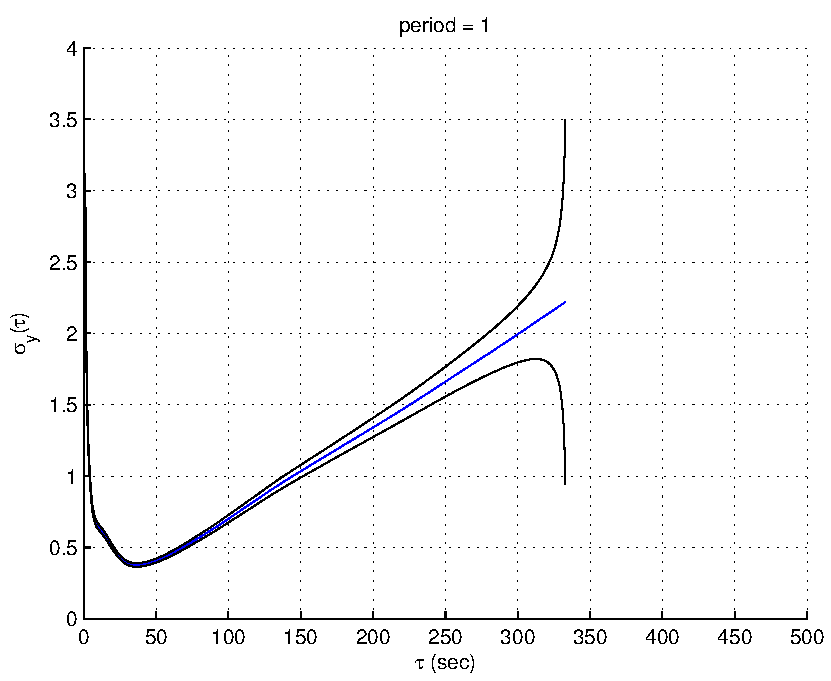
\includegraphics[width=0.7\textwidth]{alg_examples_published/MADEV_alg_example_01.pdf}
\end{center}



%%% \end{document}
    


\chapter{OADEV -- Overlapping Allan Deviation} %<<<1 ------------------------------
\chaptermark{OADEV}
% included files are automatically generated by info_all_algs.m script and by Matlab publish
% function and converted by bash script betterpublish.
\section*{\infosection} %<<<2 -------------------
\begin{tightdesc}
\item [\textsf{.id}] --- OADEV
\item [\textsf{.name}] --- Overlapping Allan Deviation
\item [\textsf{.desc}] --- Compute the overlapping Allan deviation for a set of time-domain frequency data.
\item [\textsf{.citation}] --- W. J. Riley, "The Calculation of Time Domain Frequency Stability". Implementation: M. A. Hopcroft, mhopeng@gmail.com, Matlab Central.
\item [\textsf{.remarks}] --- If tau is empty array, tau values are automatically generated. Tau values must be divisible by 1/fs. Invalid values are ignored. For tau values really used in the calculation see the output. Using sigma as uncertainty is probably not correct.
\item [\textsf{.license}] --- BSD License
\item [\textsf{.requires}] \rule{0em}{0em}
\begin{tightdesc}
\item [\textsf{y}] --- sampled values
\item [\textsf{fs}] --- sampling frequency
\item [\textsf{tau}] --- observation time
\end{tightdesc}
\item [\textsf{.returns}] \rule{0em}{0em}
\begin{tightdesc}
\item [\textsf{oadev}] --- overlapping Allan deviation
\item [\textsf{tau}] --- observation time of result values
\end{tightdesc}
\item [\textsf{.providesGUF}] --- yes
\item [\textsf{.providesMCM}] ---  no
\end{tightdesc}

\section*{\examplesection} %<<<2 ------------------------

% This LaTeX was auto-generated from an M-file by MATLAB.
% To make changes, update the M-file and republish this document.

%%% \documentclass{article}
%%% \usepackage{graphicx}
%%% \usepackage{color}

%%% \sloppy
%%% \definecolor{lightgray}{gray}{0.5}
\setlength{\parindent}{0pt}

%%% \begin{document}

    
    
\subsection*{Allan Overlapping Deviation}

\begin{par}
Example for algorithm OADEV.
\end{par} \vspace{1em}
\begin{par}
OADEV is an algorithm to compute the overlapping Allan deviation for a set of time-domain frequency data.
\end{par} \vspace{1em}
\begin{par}
See also W. J. Riley, "The Calculation of Time Domain Frequency Stability". Implementation: M. A. Hopcroft, \verb"mhopeng@gmail.com", Matlab Central.'
\end{par} \vspace{1em}

\subsubsection*{Contents}

\begin{itemize}
\setlength{\itemsep}{-1ex}
   \item Generate sample data
   \item Call algorithm
   \item Display results
\end{itemize}


\subsubsection*{Generate sample data}

\begin{lstlisting}[style=mcode]
DI = [];
%!demo
%ysin=2.*sin(2.*pi.*1/300.*[1:1:1e3]);
%! [x y s errors]=adev(1, ysin, 1, 'best averaging time is 300 s, i.e. cca one sine period');
% A random numbers with normal probability distribution function will be generated into data input |DI.y.v|.
DI.y.v = 1.5 + 3.*randn(1, 1e3);
% Next a drift is added:
DI.y.v = DI.y.v + [1:1:1e3]./100;
% Lets suppose a sampling frequency is 1 Hz:
DI.fs.v = 1;
% Let the algorithm generate all possible tau values automatically:
DI.tau.v = [];
\end{lstlisting}


\subsubsection*{Call algorithm}

\begin{par}
Use QWTB to apply algorithm \lstinline{OADEV} to data \lstinline{DI}.
\end{par} \vspace{1em}
\begin{lstlisting}[style=mcode]
DO = qwtb('OADEV', DI);
\end{lstlisting}

        \begin{lstlisting}[style=output]
QWTB: no uncertainty calculation
\end{lstlisting} \color{black}
    

\subsubsection*{Display results}

\begin{par}
Log log figure is the best to see allan deviation results:
\end{par} \vspace{1em}
\begin{lstlisting}[style=mcode]
figure; hold on
loglog(DO.tau.v, DO.oadev.v, '-b')
loglog(DO.tau.v, DO.oadev.v + DO.oadev.u, '-k')
loglog(DO.tau.v, DO.oadev.v - DO.oadev.u, '-k')
xlabel('\tau (sec)');
ylabel('\sigma_y(\tau)');
title(['period = ' num2str(DI.fs.v)]);
grid('on'); hold off
\end{lstlisting}

\begin{center}
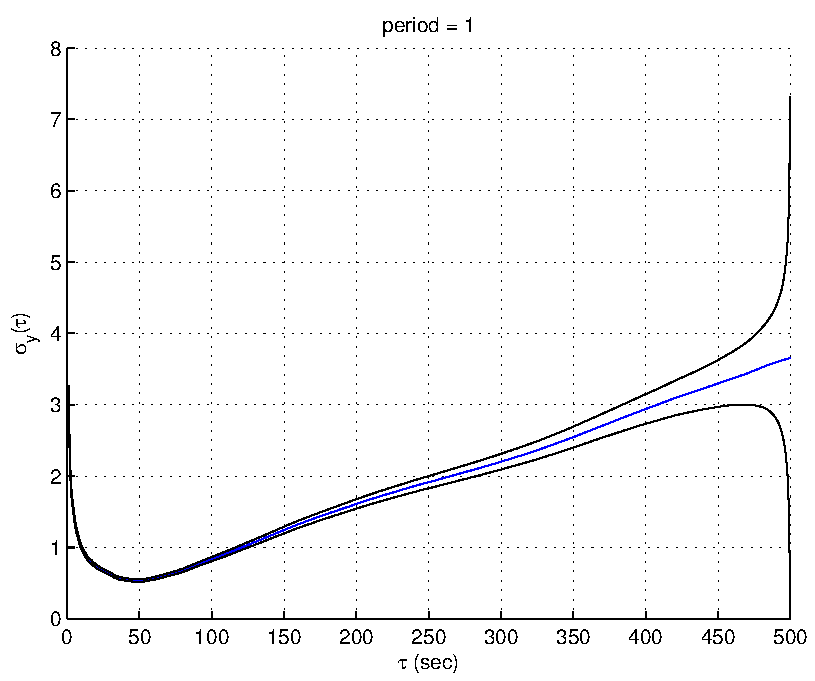
\includegraphics[width=0.7\textwidth]{algs_examples_published/OADEV_alg_example_01.pdf}
\end{center}



%%% \end{document}
    


\chapter{PSFE -- Phase Sensitive Frequency Estimator} %<<<1 ------------------------------
\chaptermark{PSFE}
% included files are automatically generated by info_all_algs.m script and by Matlab publish
% function and converted by bash script betterpublish.
\section*{\infosection} %<<<2 -------------------
\begin{tightdesc}
\item [Id:] PSFE
\item [Name:] Phase Sensitive Frequency Estimator
\item [Description:] An algorithm for estimating the frequency, amplitude, and phase of the fundamental component in harmonically distorted waveforms. The algorithm minimizes the phase difference between the sine model and the sampled waveform by effectively minimizing the influence of the harmonic components. It uses a three-parameter sine-fitting algorithm for all phase calculations. The resulting estimates show up to two orders of magnitude smaller sensitivity to harmonic distortions than the results of the four-parameter sine fitting algorithm.
\item [Citation:] Lapuh, R., "Estimating the Fundamental Component of Harmonically Distorted Signals From Noncoherently Sampled Data," Instrumentation and Measurement, IEEE Transactions on , vol.64, no.6, pp.1419,1424, June 2015, doi: 10.1109/TIM.2015.2401211, URL: \url{http://ieeexplore.ieee.org/stamp/stamp.jsp?tp=\&arnumber=7061456\&isnumber=7104190}
\item [Remarks:] If sampling time |Ts| is not supplied, wrapper will calculate |Ts| from sampling frequency |fs| or if not supplied, mean of differences of time series |t| is used to calculate |Ts|.
\item [License:] MIT License
\item [Provides GUF:] no
\item [Provides MCM:] no
\item [Input Quantities] \rule{0em}{0em}
    \begin{tightdesc}
    \item [Required:] 
        \textsf{Ts} or \textsf{fs} or \textsf{t},\enspace \textsf{y}
    \item [Descriptions:] \rule{0em}{0em}
        \begin{tightdesc}
            \item[\textsf{Ts}] -- Sampling time
            \item[\textsf{fs}] -- Sampling frequency
            \item[\textsf{t}] -- Time series
            \item[\textsf{y}] -- Sampled values
        \end{tightdesc}
    \end{tightdesc}
\item [Output Quantities:] \rule{0em}{0em}
    \begin{tightdesc}
        \item[\textsf{A}] -- Amplitude of main signal component
        \item[\textsf{f}] -- Frequency of main signal component
        \item[\textsf{ph}] -- Phase of main signal component
    \end{tightdesc}
\end{tightdesc}

\section*{\examplesection} %<<<2 ------------------------

% This LaTeX was auto-generated from an M-file by MATLAB.
% To make changes, update the M-file and republish this document.

%%% \documentclass{article}
%%% \usepackage{graphicx}
%%% \usepackage{color}

%%% \sloppy
%%% \definecolor{lightgray}{gray}{0.5}
\setlength{\parindent}{0pt}

%%% \begin{document}

    
    
\subsection*{Phase Sensitive Frequency Estimator}

\begin{par}
Example for algorithm PSFE.
\end{par} \vspace{1em}
\begin{par}
PSFE is an algorithm for estimating the frequency, amplitude, and phase of the fundamental component in harmonically distorted waveforms. The algorithm minimizes the phase difference between the sine model and the sampled waveform by effectively minimizing the influence of the harmonic components. It uses a three-parameter sine-fitting algorithm for all phase calculations. The resulting estimates show up to two orders of magnitude smaller sensitivity to harmonic distortions than the results of the four-parameter sine fitting algorithm.
\end{par} \vspace{1em}
\begin{par}
See also Lapuh, R., "Estimating the Fundamental Component of Harmonically Distorted Signals From Noncoherently Sampled Data," Instrumentation and Measurement, IEEE Transactions on , vol.64, no.6, pp.1419,1424, June 2015, doi: 10.1109/TIM.2015.2401211, URL: \url{http://ieeexplore.ieee.org/stamp/stamp.jsp?tp=&arnumber=7061456&isnumber=7104190}'
\end{par} \vspace{1em}

\subsubsection*{Contents}

\begin{itemize}
\setlength{\itemsep}{-1ex}
   \item Generate sample data
   \item Call algorithm
   \item Display results
\end{itemize}


\subsubsection*{Generate sample data}

\begin{par}
Two quantities are prepared: \lstinline{t} and \lstinline{y}, representing 1 second of sinus waveform of nominal frequency 100 Hz, nominal amplitude 1 V and nominal phase 1 rad, sampled at sampling frequency 10 kHz.
\end{par} \vspace{1em}
\begin{lstlisting}[style=mcode]
DI = [];
Anom = 1; fnom = 100; phnom = 1;
DI.t.v = [0:1/1e4:1-1/1e4];
DI.y.v = Anom*sin(2*pi*fnom*DI.t.v + phnom);
\end{lstlisting}
\begin{par}
Add noise:
\end{par} \vspace{1em}
\begin{lstlisting}[style=mcode]
DI.y.v = DI.y.v + normrnd(0, 1e-3, size(DI.y.v));
\end{lstlisting}


\subsubsection*{Call algorithm}

\begin{par}
Use QWTB to apply algorithm \lstinline{PSFE} to data \lstinline{DI}.
\end{par} \vspace{1em}
\begin{lstlisting}[style=mcode]
DO = qwtb('PSFE', DI);
\end{lstlisting}

        \begin{lstlisting}[style=output]
QWTB: no uncertainty calculation
\end{lstlisting} \color{black}
    

\subsubsection*{Display results}

\begin{par}
Results is the amplitude, frequency and phase of sampled waveform.
\end{par} \vspace{1em}
\begin{lstlisting}[style=mcode]
f = DO.f.v
A = DO.A.v
ph = DO.ph.v
\end{lstlisting}

        \begin{lstlisting}[style=output]

f =

  100.0000


A =

    1.0000


ph =

    1.0000

\end{lstlisting} \color{black}
    \begin{par}
Errors of estimation in parts per milion:
\end{par} \vspace{1em}
\begin{lstlisting}[style=mcode]
ferrppm = (DO.f.v - fnom)/fnom .* 1e6
Aerrppm = (DO.A.v - Anom)/Anom .* 1e6
pherrppm = (DO.ph.v - phnom)/phnom .* 1e6
\end{lstlisting}

        \begin{lstlisting}[style=output]

ferrppm =

    0.1113


Aerrppm =

    4.3774


pherrppm =

  -13.7952

\end{lstlisting} \color{black}
    


%%% \end{document}
    


\chapter{SFDR -- Spurious Free Dynamic Range} %<<<1 ------------------------------
\chaptermark{SFDR}
% included files are automatically generated by info_all_algs.m script and by Matlab publish
% function and converted by bash script betterpublish.
\section*{\infosection} %<<<2 -------------------
\begin{tightdesc}
\item [Id:] SFDR
\item [Name:] Spurious Free Dynamic Range
\item [Description:] Calculates Spurious Free Dynamic Range of an ADC. A FFT method with Blackman windowing is used to calculate a spectrum and SFDR is estimated in decibels relative to carrier amplitude. ADC has to sample a pure sine wave. SFDR is calculated according IEEE Std 1057-2007
\item [Citation:] Implementation: Virosztek, T., Pálfi V., Renczes B., Kollár I., Balogh L., Sárhegyi A., Márkus J., Bilau Z. T., ADCTest project site: \url{http://www.mit.bme.hu/projects/adctest} 2000-2014
\item [Remarks:] Based on the ADCTest Toolbox v4.3, November 25, 2014.
\item [License:] UNKNOWN
\item [Provides GUF:] no
\item [Provides MCM:] no
\item [Input Quantities] \rule{0em}{0em}
    \begin{tightdesc}
    \item [Required:] 
        \textsf{y}
    \end{tightdesc}
\item [Descriptions:] \rule{0em}{0em}
    \begin{tightdesc}
        \item[\textsf{y}] -- Sampled values
    \end{tightdesc}
\item [Output Quantities] \rule{0em}{0em}
    \begin{tightdesc}
        \item[\textsf{SFDRdBc}] -- Spurious Free Dynamic Range in decibels relative to carrier (dBc)
    \end{tightdesc}
\end{tightdesc}

\section*{\examplesection} %<<<2 ------------------------

% This LaTeX was auto-generated from an M-file by MATLAB.
% To make changes, update the M-file and republish this document.

%%% \documentclass{article}
%%% \usepackage{graphicx}
%%% \usepackage{color}

%%% \sloppy
%%% \definecolor{lightgray}{gray}{0.5}
\setlength{\parindent}{0pt}

%%% \begin{document}

    
    
\subsection*{Spurious Free Dynamic Range by means of Fast fourier transform}

\begin{par}
Example for algorithm SFDR.
\end{par} \vspace{1em}
\begin{par}
Calculates SFDR by calculating FFT spectrum.
\end{par} \vspace{1em}

\subsubsection*{Contents}

\begin{itemize}
\setlength{\itemsep}{-1ex}
   \item Generate sample data
   \item Call algorithm
   \item Display results
\end{itemize}


\subsubsection*{Generate sample data}

\begin{par}
First quantity \lstinline{y} representing 1 second of signal containing spurious component is prepared. Main signal component has nominal frequency 1 kHz, nominal amplitude 2 V, nominal phase 1 rad and offset 1 V sampled at sampling frequency 10 kHz.
\end{par} \vspace{1em}
\begin{lstlisting}[style=mcode]
DI = [];
fsnom = 1e4; Anom = 4; fnom = 100; phnom = 1; Onom = 0.2;
t = [0:1/fsnom:1-1/fsnom];
DI.y.v = Anom*sin(2*pi*fnom*t + phnom);
\end{lstlisting}
\begin{par}
A spurious component with amplitude at 1/100 of main carrier frequency is added. Thus by definition the SFDR in dBc has to be 40.
\end{par} \vspace{1em}
\begin{lstlisting}[style=mcode]
DI.y.v = DI.y.v + Anom./100*sin(2*pi*fnom*3.5*t + phnom);
\end{lstlisting}


\subsubsection*{Call algorithm}

\begin{par}
Use QWTB to apply algorithm \lstinline{SFDR} to data \lstinline{DI}.
\end{par} \vspace{1em}
\begin{lstlisting}[style=mcode]
DO = qwtb('SFDR', DI);
\end{lstlisting}

        \begin{lstlisting}[style=output]
QWTB: no uncertainty calculation
\end{lstlisting} \color{black}
    

\subsubsection*{Display results}

\begin{par}
Result is the SFDR (dBc).
\end{par} \vspace{1em}
\begin{lstlisting}[style=mcode]
SFDR = DO.SFDRdBc.v
\end{lstlisting}

        \begin{lstlisting}[style=output]

SFDR =

   40.0000

\end{lstlisting} \color{black}
    


%%% \end{document}
    


\chapter{SINAD-ENOB -- Ratio of signal to noise and distortion and Effective number of bits (in time space)} %<<<1 ------------------------------
\chaptermark{SINAD-ENOB}
% included files are automatically generated by info_all_algs.m script and by Matlab publish
% function and converted by bash script betterpublish.
\section*{\infosection} %<<<2 -------------------
\begin{tightdesc}
\item [Id:] SINAD-ENOB
\item [Name:] Ratio of signal to noise and distortion and Effective number of bits (in time space)
\item [Description:]  Algorithm calculates Ratio of signal to noise and distortion and Effective number of bits in time space, therefore it is suitable for noncoherent measurements. Requires estimates of the main signal component parameters: frequency, amplitude, phase and offset. If these values are estimated by four parameter sine wave fit, the SINAD and ENOB will be calculated according IEEE Std 1241-2000. A large sine wave should be applied to the ADC input. Almost any error source in the sine wave input other than gain accuracy and dc offset can affect the test result.
\item [Citation:] IEEE Std 1241-2000, pages 52 - 54
\item [Remarks:] If Time series |t| is not supplied, wrapper will calculate |t| from sampling frequency |fs| or if not supplied, sampling time |Ts| is used to calculate |t|.
\item [License:] MIT License
\item [Provides GUF:] no
\item [Provides MCM:] no
\item [Input Quantities] \rule{0em}{0em}
    \begin{tightdesc}
    \item [Required:] 
        \textsf{t} or \textsf{fs} or \textsf{Ts},\enspace \textsf{y},\enspace \textsf{f},\enspace \textsf{A},\enspace \textsf{ph},\enspace \textsf{O},\enspace \textsf{bitres},\enspace \textsf{FSR}
    \end{tightdesc}
\item [Descriptions:] \rule{0em}{0em}
    \begin{tightdesc}
        \item[\textsf{A}] -- Amplitude of main signal component
        \item[\textsf{FSR}] -- Full scale range of an ADC
        \item[\textsf{O}] -- Offset of signal
        \item[\textsf{Ts}] -- Sampling time
        \item[\textsf{bitres}] -- Bit resolution of an ADC
        \item[\textsf{f}] -- Frequency of main signal component
        \item[\textsf{fs}] -- Sampling frequency
        \item[\textsf{ph}] -- Phase of main signal component
        \item[\textsf{t}] -- Time series
        \item[\textsf{y}] -- Sampled values
    \end{tightdesc}
\item [Output Quantities] \rule{0em}{0em}
    \begin{tightdesc}
        \item[\textsf{ENOB}] -- Effective number of bits
        \item[\textsf{SINADdB}] -- Ratio of signal to noise and distortion in decibels relative to the amplitude of the main signal component
    \end{tightdesc}
\end{tightdesc}

\section*{\examplesection} %<<<2 ------------------------

% This LaTeX was auto-generated from an M-file by MATLAB.
% To make changes, update the M-file and republish this document.

%%% \documentclass{article}
%%% \usepackage{graphicx}
%%% \usepackage{color}

%%% \sloppy
%%% \definecolor{lightgray}{gray}{0.5}
\setlength{\parindent}{0pt}

%%% \begin{document}

    
    
\subsection*{Ratio of signal to noise and distortion and Effective number of bits (time space)}

\begin{par}
Example for algorithm SINAD-ENOB.
\end{par} \vspace{1em}
\begin{par}
Algorithm calculates Ratio of signal to noise and distortion and Effective number of bits in time space. First signal is generated, then estimates of signal parameters are calculated by Four parameter sine wave fitting and next SINAD and ENOB are calculated. This example do not take into account a quantisation noise.
\end{par} \vspace{1em}

\subsubsection*{Contents}

\begin{itemize}
\setlength{\itemsep}{-1ex}
   \item Generate sample data
   \item Calculate estimates of signal parameters
   \item Copy results to inputs
   \item Calculate SINAD and ENOB
   \item Display results:
\end{itemize}


\subsubsection*{Generate sample data}

\begin{par}
Two quantities are prepared: \lstinline{t} and \lstinline{y}, representing 1 second of sinus waveform of nominal frequency 1 kHz, nominal amplitude 1 V, nominal phase 1 rad and offset 1 V sampled at sampling frequency 10 kHz.
\end{par} \vspace{1em}
\begin{lstlisting}[style=mcode]
DI = [];
Anom = 2; fnom = 100; phnom = 1; Onom = 0.2;
DI.t.v = [0:1/1e4:1-1/1e4];
DI.y.v = Anom*sin(2*pi*fnom*DI.t.v + phnom) + Onom;
\end{lstlisting}
\begin{par}
Add a noise with normal distribution probability:
\end{par} \vspace{1em}
\begin{lstlisting}[style=mcode]
noisestd = 1e-4;
DI.y.v = DI.y.v + noisestd.*randn(size(DI.y.v));
\end{lstlisting}
\begin{par}
Lets make an estimate of frequency 0.2 percent higher than nominal value:
\end{par} \vspace{1em}
\begin{lstlisting}[style=mcode]
DI.fest.v = 100.2;
\end{lstlisting}


\subsubsection*{Calculate estimates of signal parameters}

\begin{par}
Use QWTB to apply algorithm \lstinline{FPSWF} to data \lstinline{DI}.
\end{par} \vspace{1em}
\begin{lstlisting}[style=mcode]
CS.verbose = 1;
DO = qwtb('FPSWF', DI, CS);
\end{lstlisting}

        \begin{lstlisting}[style=output]
QWTB: no uncertainty calculation
Fitting started

Local minimum found.

Optimization completed because the size of the gradient is less than
the default value of the function tolerance.



Fitting finished
\end{lstlisting} \color{black}
    

\subsubsection*{Copy results to inputs}

\begin{par}
Take results of \lstinline{FPSWF} and put them as inputs \lstinline{DI}.
\end{par} \vspace{1em}
\begin{lstlisting}[style=mcode]
DI.f = DO.f;
DI.A = DO.A;
DI.ph = DO.ph;
DI.O = DO.O;
\end{lstlisting}
\begin{par}
Suppose the signal was sampled by a 20 bit digitizer with full scale range of 6 V (+- 3V). (The signal is not quantised, so the quantization noise is not present. Thus the simulation and results are not fully correct.):
\end{par} \vspace{1em}
\begin{lstlisting}[style=mcode]
DI.bitres.v = 20;
DI.range.v = 3;
\end{lstlisting}


\subsubsection*{Calculate SINAD and ENOB}

\begin{lstlisting}[style=mcode]
DO = qwtb('SINAD-ENOB', DI, CS);
\end{lstlisting}

        \begin{lstlisting}[style=output]
QWTB: no uncertainty calculation
\end{lstlisting} \color{black}
    

\subsubsection*{Display results:}

\begin{par}
Results are:
\end{par} \vspace{1em}
\begin{lstlisting}[style=mcode]
SINADdB = DO.SINADdB.v
ENOB = DO.ENOB.v
\end{lstlisting}

        \begin{lstlisting}[style=output]

SINADdB =

   83.0029


ENOB =

   13.0790

\end{lstlisting} \color{black}
    \begin{par}
Theoretical value of SINADdB is 20*log10(Anom./(noisestd.*sqrt(2))). Theoretical value of ENOB is log2(DI.range.v./(noisestd.*sqrt(12))). Absolute error of results are:
\end{par} \vspace{1em}
\begin{lstlisting}[style=mcode]
SINADdBtheor = 20*log10(Anom./(noisestd.*sqrt(2)));
ENOBtheor = log2(DI.range.v./(noisestd.*sqrt(12)));
SINADerror = SINADdB - SINADdBtheor
ENOBerror = ENOB - ENOBtheor
\end{lstlisting}

        \begin{lstlisting}[style=output]

SINADerror =

   -0.0074


ENOBerror =

   -0.0012

\end{lstlisting} \color{black}
    


%%% \end{document}
    


\chapter{SP-FFT -- Spectrum by means of Fast Fourier Transform} %<<<1 ------------------------------
\chaptermark{SP-FFT}
% included files are automatically generated by info_all_algs.m script and by Matlab publish
% function and converted by bash script betterpublish.
\section*{\infosection} %<<<2 -------------------
\begin{tightdesc}
\item [\textsf{.id}] --- SP-FFT
\item [\textsf{.name}] --- Spectrum by means of Fast Fourier Transform
\item [\textsf{.desc}] --- Calculates frequency and phase spectrum by means of Fast Fourier Transform algorithm. Result is normalized.
\item [\textsf{.citation}] --- 
\item [\textsf{.remarks}] --- 
\item [\textsf{.license}] --- MIT License
\item [\textsf{.requires}] \rule{0em}{0em}
\begin{tightdesc}
\item [\textsf{y}] --- Sampled values
\item [\textsf{fs}] --- Sampling frequency
\end{tightdesc}
\item [\textsf{.returns}] \rule{0em}{0em}
\begin{tightdesc}
\item [\textsf{f}] --- Frequency series
\item [\textsf{A}] --- Amplitude series
\item [\textsf{ph}] --- Phase series
\end{tightdesc}
\item [\textsf{.providesGUF}] --- no
\item [\textsf{.providesMCM}] ---  no
\end{tightdesc}

\section*{\examplesection} %<<<2 ------------------------

% This LaTeX was auto-generated from an M-file by MATLAB.
% To make changes, update the M-file and republish this document.

%%% \documentclass{article}
%%% \usepackage{graphicx}
%%% \usepackage{color}

%%% \sloppy
%%% \definecolor{lightgray}{gray}{0.5}
\setlength{\parindent}{0pt}

%%% \begin{document}

    
    
\subsection*{Signal Spectrum by means of Fast fourier transform}

\begin{par}
Example for algorithm SP-FFT.
\end{par} \vspace{1em}
\begin{par}
Calculates frequency and phase spectrum by means of Fast Fourier Transform algorithm. Result is normalized.
\end{par} \vspace{1em}

\subsubsection*{Contents}

\begin{itemize}
\setlength{\itemsep}{-1ex}
   \item Generate sample data
   \item Call algorithm
   \item Display results
\end{itemize}


\subsubsection*{Generate sample data}

\begin{par}
Two quantities are prepared: \lstinline{y} and \lstinline{fs}, representing 1 second of signal containing 5 harmonic components and one inter-harmonic component. Main signal component has nominal frequency 1 kHz, nominal amplitude 2 V, nominal phase 1 rad and offset 1 V sampled at sampling frequency 10 kHz.
\end{par} \vspace{1em}
\begin{lstlisting}[style=mcode]
DI = [];
fsnom = 1e4; Anom = 2; fnom = 100; phnom = 1; Onom = 0.2;
t = [0:1/fsnom:1-1/fsnom];
DI.y.v = Anom*sin(2*pi*fnom*t + phnom);
for i = 2:45
        DI.y.v = DI.y.v + Anom./i*sin(2*pi*fnom*i*t + phnom + i - 1);
end
DI.y.v = DI.y.v + 1*sin(2*pi*fnom*1.456*t + phnom);
DI.fs.v = fsnom;
\end{lstlisting}


\subsubsection*{Call algorithm}

\begin{par}
Use QWTB to apply algorithm \lstinline{SP-FFT} to data \lstinline{DI}.
\end{par} \vspace{1em}
\begin{lstlisting}[style=mcode]
DO = qwtb('SP-FFT', DI);
\end{lstlisting}

        \begin{lstlisting}[style=output]
QWTB: no uncertainty calculation
\end{lstlisting} \color{black}
    

\subsubsection*{Display results}

\begin{par}
Results is the amplitude and phase spectrum.
\end{par} \vspace{1em}
\begin{lstlisting}[style=mcode]
figure
plot(DO.f.v, DO.A.v, '-x')
xlabel('f (Hz)'); ylabel('A (V)'); title('Amplitude spectrum of the signal');
figure
plot(DO.f.v, DO.ph.v, '-x')
xlabel('f (Hz)'); ylabel('phase (rad)'); title('Phase spectrum of the signal');
\end{lstlisting}

\begin{center}
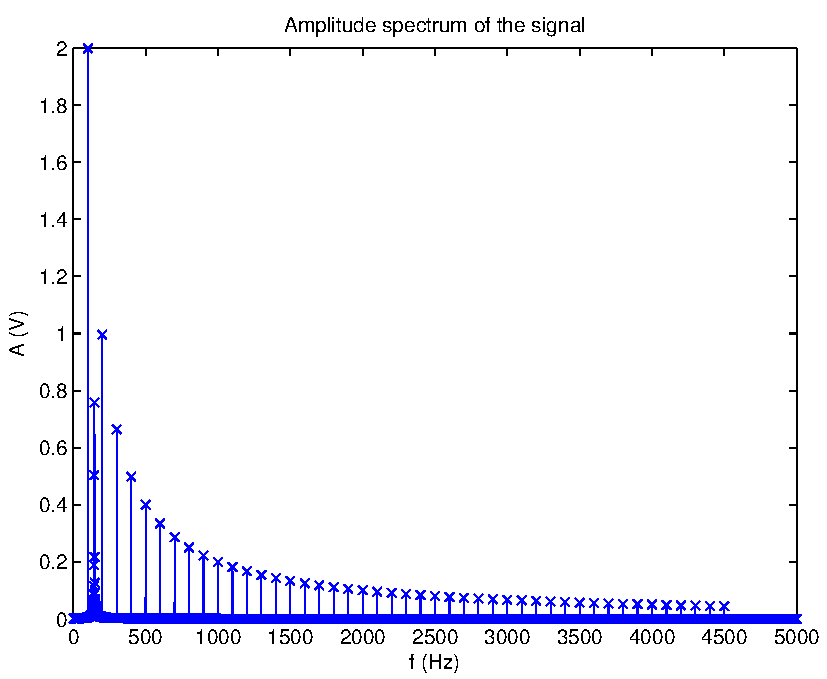
\includegraphics[width=0.7\textwidth]{algs_examples_published/SP-FFT_alg_example_01.pdf}
\end{center}

\begin{center}
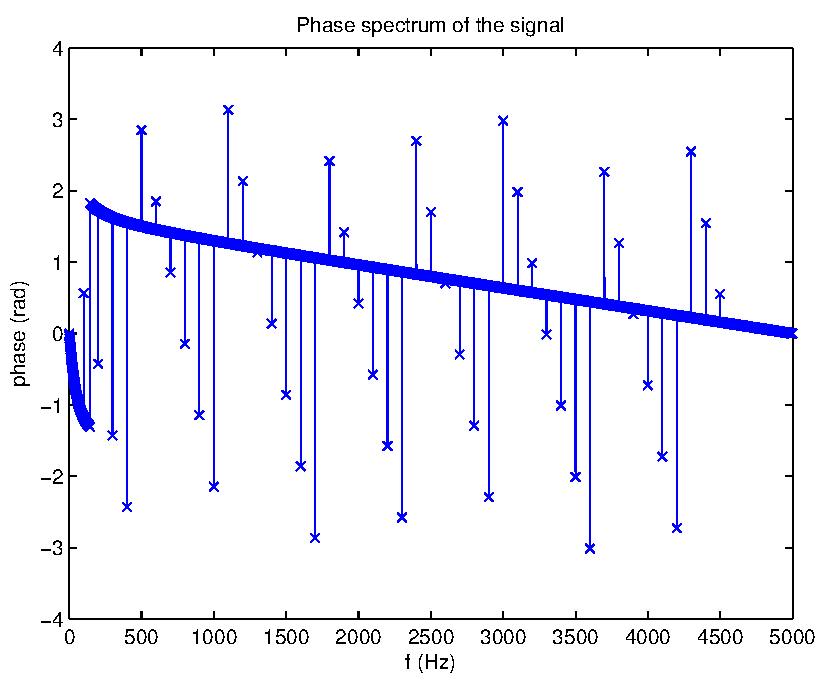
\includegraphics[width=0.7\textwidth]{algs_examples_published/SP-FFT_alg_example_02.pdf}
\end{center}



%%% \end{document}
    


\chapter{SP-WFFT -- Spectrum by means of Windowed Discrete Fourier Transform} %<<<1 ------------------------------
\chaptermark{SP-WFFT}
% included files are automatically generated by info_all_algs.m script and by Matlab publish
% function and converted by bash script betterpublish.
\section*{\infosection} %<<<2 -------------------
\begin{tightdesc}
\item [Id:] SP-WFFT
\item [Name:] Spectrum by means of Windowed Discrete Fourier Transform
\item [Description:] Calculates amplitude and phase spectrum by means of Discrete Fourier Transform with windowing and/or zero padding. Result is normalized. Follwing windows are implemented: barthann, bartlett, blackman, blackmanharris, blackmannuttall, bohman, cheb, flattop\_matlab, flattop\_SFT3F, flattop\_SFT4F, flattop\_SFT5F, flattop\_SFT3M, flattop\_SFT4M, flattop\_SFT5M, flattop\_248D, gaussian, hamming, hanning, kaiser, nuttall, parzen, rect, triang, tukey, welch.
\item [Citation:]  Various sources. See algorithm scripts for details. A. V. Oppenheim and R. W. Schafer, Discrete-Time Signal Processing. Peter Lynch, "The Dolph-Chebyshev Window: A Simple Optimal Filter", Monthly Weather Review, Vol. 125, pp. 655-660, April 1997, \url{http://www.maths.tcd.ie/~plynch/Publications/Dolph.pdf} . C. Dolph, "A current distribution for broadside arrays which optimizes the relationship between beam width and side-lobe level", Proc. IEEE, 34, pp. 335-348. \url{https://www.mathworks.com/help/signal/ref/flattopwin.html} . D`Antona, Gabriele, and A. Ferrero. Digital Signal Processing for Measurement Systems. New York: Springer Media, 2006, pp. 70–72. Gade, Svend, and Henrik Herlufsen. "Use of Weighting Functions in DFT/FFT Analysis (Part I)." Windows to FFT Analysis (Part I): Bruel and Kjaer Technical Review, No. 3, 1987, pp. 1-28. G. Heinzel, `Spectrum and spectral density estimation by the Discrete Fourier transform (DFT), including a comprehensive list of window functions and some new flat-top windows`, IEEE, 2003. Fredric J. Harris, "On the Use of Windows for Harmonic Analysis with the Discrete Fourier Transform, Proceedings of the IEEE", Vol. 66, No. 1, January 1978, Page 67, Equation 38. Implemented by: Sylvain Pelissier, Andreas Weingessel, Muthiah Annamalai, Andre Carezia, Vera Novaková Zachovalova, Paul Kienzle, Paul Kienzle, Laurent Mazet, Muthiah Annamalai, Mike Gross, Peter V. Lanspeary.
\item [Remarks:] If sampling frequency |fs| is not supplied, wrapper will calculate |fs| from sampling time |Ts| or if not supplied, first two elements of time series |t| are used to calculate |fs|. If |window| is not specified, a rectangular (none) window will be used. If |window| is `cheb` and |cheb\_att| is not specified, a value of 100 dB is set. If |window| is `gaussian` and |gaussian\_width| is not specified, a value of 1 is set. If |window| is `kaiser` and |kaiser\_att| is not specified, a value of 0.5 is set. If |window| is `tukey` and |tukey\_ratio| is not specified, a value of 0.5 is set.
\item [License:] Mixed license - every window function has its own license.
\item [Provides GUF:] no
\item [Provides MCM:] no
\item [Input Quantities] \rule{0em}{0em}
    \begin{tightdesc}
    \item [Required:] 
        \textsf{fs} or \textsf{Ts} or \textsf{t},\enspace \textsf{y}
    \item [Optional:] 
        \textsf{window},\enspace \textsf{cheb\_att},\enspace \textsf{gaussian\_width},\enspace \textsf{kaiser\_att},\enspace \textsf{fft\_padding}
    \item [Parameters:] 
        \textsf{window},\enspace \textsf{cheb\_att},\enspace \textsf{gaussian\_width},\enspace \textsf{kaiser\_att},\enspace \textsf{fft\_padding}
    \item [Descriptions:] \rule{0em}{0em}
        \begin{tightdesc}
            \item[\textsf{Ts}] -- Sampling time
            \item[\textsf{cheb\_att}] -- Only for Dolph-Chebyshev window: stop-band attenuation in dB
            \item[\textsf{fft\_padding}] -- Zero padding of signal in samples
            \item[\textsf{fs}] -- Sampling frequency
            \item[\textsf{gaussian\_width}] -- Only for Gaussian window: width of the window in Hz
            \item[\textsf{kaiser\_att}] -- Only for Kaiser window: stop-band attenuation in FFT bins
            \item[\textsf{t}] -- Time series
            \item[\textsf{window}] -- Name of window function
            \item[\textsf{y}] -- Sampled values
        \end{tightdesc}
    \end{tightdesc}
\item [Output Quantities:] \rule{0em}{0em}
    \begin{tightdesc}
        \item[\textsf{A}] -- Amplitude spectrum
        \item[\textsf{f}] -- Frequency series
        \item[\textsf{ph}] -- Phase spectrum
    \end{tightdesc}
\end{tightdesc}

\section*{\examplesection} %<<<2 ------------------------

% This LaTeX was auto-generated from an M-file by MATLAB.
% To make changes, update the M-file and republish this document.

%%% \documentclass{article}
%%% \usepackage{graphicx}
%%% \usepackage{color}

%%% \sloppy
%%% \definecolor{lightgray}{gray}{0.5}
\setlength{\parindent}{0pt}

%%% \begin{document}

    
    
\subsection*{Windowed Discrete Fourier Transform}

\begin{par}
Example for algorithm SP-WFFT.
\end{par} \vspace{1em}
\begin{par}
Windowed Discrete Fourier Transform is method to calculate frequency and phase spectrum. Example shows the effect of coherent sampling, non-coherent sampling, windowing and zero padding on estimating amplitude and phase by means of FFT. Last part compares all windows in frequency space.
\end{par} \vspace{1em}

\subsubsection*{Contents}

\begin{itemize}
\setlength{\itemsep}{-1ex}
   \item Generate sample data
   \item Call algorithm
   \item Display results
   \item Compare window coefficients
\end{itemize}


\subsubsection*{Generate sample data}

\begin{par}
Construct 1 second of signal sampled at 50 Hz containing two harmonic components at 1 and 8 Hz and one interharmonic component at 15.5 Hz with various amplitudes and phases.
\end{par} \vspace{1em}
\begin{lstlisting}[style=mcode]
clear DI
DI.fs.v = 50;
fnom = [1;   8; 15.5];
Anom = [1; 0.5;  0.3];
pnom = [0;   1;    2];
DI.t.v = [0 : 1/DI.fs.v : 1 - 1/DI.fs.v];
DI.y.v = zeros(size(DI.t.v));
for i = 1:length(fnom)
        DI.y.v = DI.y.v + Anom(i).*sin(2.*pi.*fnom(i).*DI.t.v + pnom(i));
end
%
\end{lstlisting}


\subsubsection*{Call algorithm}

\begin{par}
Calculate amplitude and phase spectrum and store results into \lstinline{DO}. Window function is not specified, therefore rectangle (none) window will be used.
\end{par} \vspace{1em}
\begin{lstlisting}[style=mcode]
DO = qwtb('SP-WFFT', DI);
%
% Set window function to blackman and calculate windowed amplitude and phase spectrum and store results into |DOw|.
DI.window.v = 'blackman';
DOw = qwtb('SP-WFFT', DI);
%
% Set zero padding to 10 times the signal length and calculate zero padded windowed amplitude and
% phase spectrum and stre results into |DOwz|.
DI.fft_padding.v = 10.*length(DI.y.v);
DOwz = qwtb('SP-WFFT', DI);
%
\end{lstlisting}

        \begin{lstlisting}[style=output]
QWTB: no uncertainty calculation
QWTB: no uncertainty calculation
QWTB: no uncertainty calculation
\end{lstlisting} \color{black}
    

\subsubsection*{Display results}

\begin{par}
Plot amplitude spectrum.
\end{par} \vspace{1em}
\begin{lstlisting}[style=mcode]
figure; hold on;
plot(fnom, Anom, '+r', 'markersize', 10, 'linewidth', 2);
stem(DO.f.v, DO.A.v, '-ob', 'filled', 'markersize', 3);
plot(DOw.f.v, DOw.A.v, '-g','linewidth',2);
plot(DOwz.f.v, DOwz.A.v, '-k');
legend('nominal values','FFT', 'blackman window', 'blck. w. + zero padding')
title('Amplitude spectrum')
xlabel('frequency (Hz)'); ylabel('amplitude (V)');
hold off
% Plot phase spectrum
figure; hold on;
plot(fnom, pnom, '+r', 'markersize', 10, 'linewidth', 2);
stem(DO.f.v, DO.ph.v, '-ob', 'filled', 'markersize', 3);
plot(DOw.f.v, DOw.ph.v, '-g','linewidth',2);
plot(DOwz.f.v, DOwz.ph.v, '-k');
legend('nominal values','FFT', 'blackman window', 'blck. w. + zero padding', 'location', 'southwest')
title('Phase spectrum');
xlabel('frequency (Hz)'); ylabel('phase (rad)');
hold off
%
\end{lstlisting}

\begin{center}
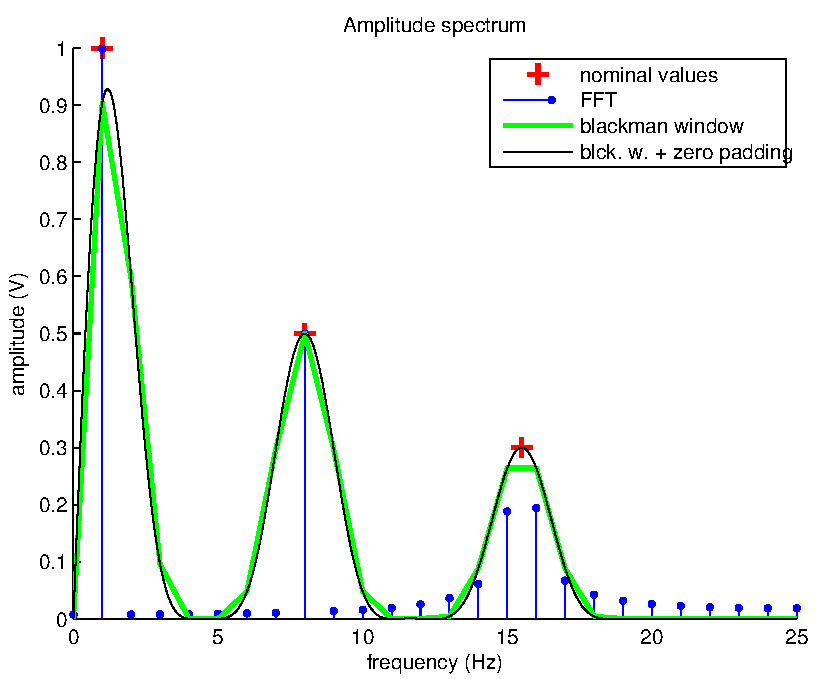
\includegraphics[width=0.7\textwidth]{algs_examples_published/SP-WFFT_alg_example_01.pdf}
\end{center}

\begin{center}
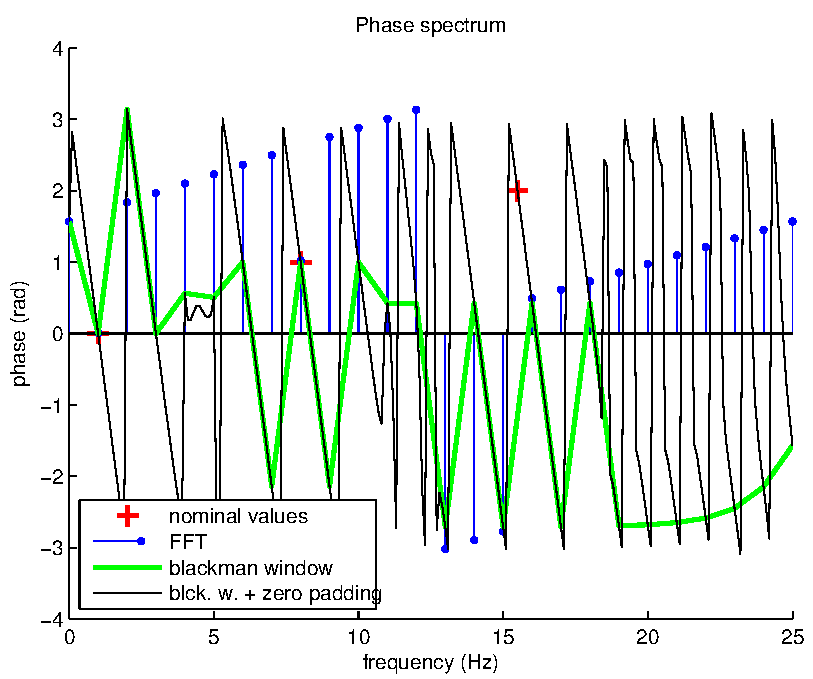
\includegraphics[width=0.7\textwidth]{algs_examples_published/SP-WFFT_alg_example_02.pdf}
\end{center}


\subsubsection*{Compare window coefficients}

\begin{par}
Different windows has different peak widths, heights of side lobes and side lobes roll off ratio. To see the window differences a zero padding is used. First a simple signal of ones is prepared and zero padding is specified to 100x the length of signal. Next for every window a spectrum is calculated and plotted.
\end{par} \vspace{1em}
\begin{lstlisting}[style=mcode]
clear DI
DI.y.v = ones(1,10);
DI.fs.v = 1;
DI.fft_padding.v = 100.*length(DI.y.v);
avail_windows = {'barthann' 'bartlett' 'blackman' 'blackmanharris' 'blackmannuttall' 'bohman' 'cheb' 'flattop_matlab' 'flattop_SFT3F' 'flattop_SFT4F' 'flattop_SFT5F' 'flattop_SFT3M' 'flattop_SFT4M' 'flattop_SFT5M' 'flattop_248D' 'gaussian' 'hamming' 'hanning' 'kaiser' 'nuttall' 'parzen' 'rect' 'triang' 'tukey' 'welch'};
col = jet(length(avail_windows));
figure; hold on;
for i = 1:length(avail_windows)
        DI.window.v = avail_windows{i};
        DO = qwtb('SP-WFFT', DI);
        plot(DO.A.v, '-', 'color', col(i,:));
end
h=legend(avail_windows);
h=legend('location','eastoutside');
set(h,'FontSize',8, 'interpreter','none');
xlabel('FFT bin * 100');
ylabel('amplitude');
hold off;
\end{lstlisting}

        \begin{lstlisting}[style=output]
QWTB: no uncertainty calculation
QWTB: no uncertainty calculation
QWTB: no uncertainty calculation
QWTB: no uncertainty calculation
QWTB: no uncertainty calculation
QWTB: no uncertainty calculation
QWTB: no uncertainty calculation
QWTB: no uncertainty calculation
QWTB: no uncertainty calculation
QWTB: no uncertainty calculation
QWTB: no uncertainty calculation
QWTB: no uncertainty calculation
QWTB: no uncertainty calculation
QWTB: no uncertainty calculation
QWTB: no uncertainty calculation
QWTB: no uncertainty calculation
QWTB: no uncertainty calculation
QWTB: no uncertainty calculation
QWTB: no uncertainty calculation
QWTB: no uncertainty calculation
QWTB: no uncertainty calculation
QWTB: no uncertainty calculation
QWTB: no uncertainty calculation
QWTB: no uncertainty calculation
QWTB: no uncertainty calculation
\end{lstlisting} \color{black}
    
\begin{center}
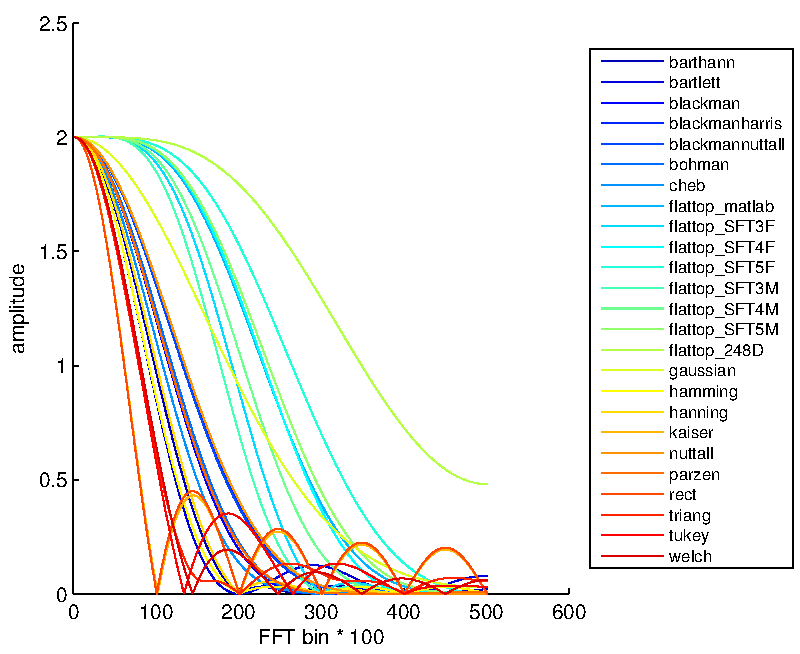
\includegraphics[width=0.7\textwidth]{algs_examples_published/SP-WFFT_alg_example_03.pdf}
\end{center}



%%% \end{document}
    


\end{document}

% vim settings: vim:foldmarker=%<<<,%>>> fdm=marker fen
\chapter{ThreePSF -- Standard Three Parameter Sine Wave Fit according IEEE Std 1241-2000} %<<<1 ------------------------------
\chaptermark{ThreePSF}
% included files are automatically generated by info_all_algs.m script and by Matlab publish
% function and converted by bash script betterpublish.
\section*{\infosection} %<<<2 -------------------
\begin{tightdesc}
\item [Id:] ThreePSF
\item [Name:] Standard Three Parameter Sine Wave Fit according IEEE Std 1241-2000
\item [Description:] Fits a sine wave to the recorded data using 3 parameter (amplitude, phase and offset) model. The algorithm is according IEEE Standard for Terminology and Test methods for Analog-to-Digital Converters 1241-2000. Algorithm requires exact value of signal frequency.
\item [Citation:] IEEE Std 1241-2000, Implementation written Rado Lapuh, 2016
\item [Remarks:] If sampling time |Ts| is not supplied, wrapper will calculate |Ts| from sampling frequency |fs| or if not supplied, mean of differences of time series |t| is used to calculate |Ts|.
\item [License:] UNKNOWN
\item [Provides GUF:] no
\item [Provides MCM:] no
\item [Input Quantities] \rule{0em}{0em}
    \begin{tightdesc}
    \item [Required:] 
        \textsf{Ts} or \textsf{fs} or \textsf{t},\enspace \textsf{f}
    \item [Descriptions:] \rule{0em}{0em}
        \begin{tightdesc}
            \item[\textsf{Ts}] -- Sampling time
            \item[\textsf{f}] -- Signal frequency
            \item[\textsf{fs}] -- Sampling frequency
            \item[\textsf{t}] -- Time series
        \end{tightdesc}
    \end{tightdesc}
\item [Output Quantities:] \rule{0em}{0em}
    \begin{tightdesc}
        \item[\textsf{A}] -- Amplitude of main signal component
        \item[\textsf{O}] -- Offset of signal
        \item[\textsf{ph}] -- Phase of main signal component
    \end{tightdesc}
\end{tightdesc}

\section*{\examplesection} %<<<2 ------------------------

% This LaTeX was auto-generated from an M-file by MATLAB.
% To make changes, update the M-file and republish this document.

%%% \documentclass{article}
%%% \usepackage{graphicx}
%%% \usepackage{color}

%%% \sloppy
%%% \definecolor{lightgray}{gray}{0.5}
\setlength{\parindent}{0pt}

%%% \begin{document}

    
    
\subsection*{Four parameter sine wave fitting}

\begin{par}
Example for algorithm ThreePSF.
\end{par} \vspace{1em}
\begin{par}
ThreePSF is an algorithm for estimating the amplitude, phase and offset of the sine waveform according standard IEEE Std 1241-2000';
\end{par} \vspace{1em}

\subsubsection*{Contents}

\begin{itemize}
\setlength{\itemsep}{-1ex}
   \item Generate sample data
   \item Call algorithm
   \item Display results
\end{itemize}


\subsubsection*{Generate sample data}

\begin{par}
Two quantities are prepared: \lstinline{t} and \lstinline{y}, representing 1 second of sinus waveform of nominal frequency 1 kHz, nominal amplitude 1 V, nominal phase 1 rad and offset 1 V sampled at sampling frequency 10 kHz.
\end{par} \vspace{1em}
\begin{lstlisting}[style=mcode]
DI = [];
Anom = 2; fnom = 100; phnom = 1; Onom = 0.2;
t = [0:1/1e4:1-1/1e4];
DI.y.v = Anom*sin(2*pi*fnom*t + phnom) + Onom;
DI.Ts.v = 1e-4;
DI.f.v = fnom;
\end{lstlisting}


\subsubsection*{Call algorithm}

\begin{par}
Use QWTB to apply algorithm \lstinline{ThreePSF} to data \lstinline{DI}.
\end{par} \vspace{1em}
\begin{lstlisting}[style=mcode]
CS.verbose = 1;
DO = qwtb('ThreePSF', DI, CS);
\end{lstlisting}

        \begin{lstlisting}[style=output]
QWTB: no uncertainty calculation
\end{lstlisting} \color{black}
    

\subsubsection*{Display results}

\begin{par}
Results is the amplitude, phase and offset of sampled waveform.
\end{par} \vspace{1em}
\begin{lstlisting}[style=mcode]
A = DO.A.v
ph = DO.ph.v
O = DO.O.v
\end{lstlisting}

        \begin{lstlisting}[style=output]

A =

    2.0000


ph =

    1.0000


O =

    0.2000

\end{lstlisting} \color{black}
    \begin{par}
Errors of estimation in parts per milion:
\end{par} \vspace{1em}
\begin{lstlisting}[style=mcode]
Aerrppm = (DO.A.v - Anom)/Anom .* 1e6
pherrppm = (DO.ph.v - phnom)/phnom .* 1e6
Oerrppm = (DO.O.v - Onom)/Onom .* 1e6
\end{lstlisting}

        \begin{lstlisting}[style=output]

Aerrppm =

  -8.4377e-09


pherrppm =

  -9.7700e-09


Oerrppm =

   8.3267e-10

\end{lstlisting} \color{black}
    


%%% \end{document}
    


